%% ----------------------------------------------------------------
%% Report.tex
%% ---------------------------------------------------------------- 
%TC:macro \inote 1
\documentclass{ecsproject}      % Use the Report Style
\graphicspath{{./Figures/}}   % Location of your graphics files
\usepackage{natbib}            % Use Natbib style for the refs.
\usepackage[nodayofweek]{datetime}
%\usepackage{todonotes}
\usepackage{longtable}
\usepackage{multirow}
\usepackage{color}
\usepackage{booktabs}
\newcommand{\inote}[1] {\todo[inline]{#1}}
\newcommand{\itc}{$I^{2}C$ }
\usepackage[disable]{todonotes}
\usepackage[intoc]{nomencl}
\usepackage{pdfpages}
\removecolourlinks
\makenomenclature
\renewcommand{\nomname}{List of Abbreviations}
%\hypersetup{colorlinks=false}   % Set to false for black/white printing
\input{Definitions}            % Include your abbreviations


%% ----------------------------------------------------------------
\begin{document}
%TC:ignore
\frontmatter
\title      {A Stereoscopic Vision Robot}
\authors    {\texorpdfstring
             {\href{mailto:hl13g10@ecs.soton.ac.uk}{Henry S. Lovett}}
             {Henry S. Lovett}
            }
\department  {Electronics and Computer Science}
\group       {Electronic and Software Systems}
\faculty{Faculty of Physical Sciences and Engineering}
\addresses  {\groupname\\\deptname\\\univname}
\date       {\today}
\subject    {}
\keywords   {}
\supervisor {Prof. Steve Gunn}
\examiner   {Prof. Mark Zwolinski}
\degree     {MEng Electronic Engineering}
\maketitle
\inote{Turn off iNotes!}

\begin{abstract}
\inote{I don't like this. Consider changing...}
This report describes the research, design, build and test of a stereoscopic vision robot using two cameras and an Atmel microcontroller. A custom PCB was designed to fit a wheeled base. 

The report is in two main parts, hardware design and vision algorithms. The hardware design section describes the prototypes and design of the subsystems.
The vision algorithms section discusses range finding from stereo images, comparison algorithms between stereo pairs, and the implementation and test of a two dimensional fast Fourier transform on an AVR. 

The final product is a small mobile robot equipped with cameras and the capability of image processing. The device has the ability to execute a predefined set of commands in an automatic stand-alone way. The robot can also be used as a shell terminal to debug and control.
\end{abstract}

%TC:ignore
\tableofcontents
\listoffigures
\listoftables
\lstlistoflistings
\clearpage
\markboth{\nomname}{\nomname}
\printnomenclature 
\cleardoublepage
\listofsymbols{ll}{
$B$ 					&	Separation distance of two cameras \\
$C_b$					&	$2\pi r_b$ \\
$C_w$					&	Circumference of the wheel \\
$D$						&	Distance from camera to the object \\
$i,j$  					&	Pixel index of an image 	\\
$r_b$					&	Distance from centre of the robot to the wheel \\
$x_0$					&	Horizontal resolution of the image \\
$x_1, x_2$				&	Distance of object from the normal of the camera \\
$\gamma$				&	Number of tabs on the wheel \\
$\Delta_\delta$			&	Distance Resolution \\
$\Delta_\Theta$			&	Rotational Resolution \\
$\delta$				& 	Distance to move \\
$\Theta$				&	Angle of rotation \\
$\sigma$				&	Standard Deviation \\
$\varphi_0$				&	Field of view of the camera \\
$\varphi_1, \varphi_2$	&	Angle from camera to the object \\
}
\nomenclature{CSV}{Comma Separated Value}
\nomenclature{DSP}{Digital Signal Processing}
\nomenclature{EBI}{External Bus Interface}
\nomenclature{USB}{Universal Serial Bus}
\nomenclature{PID}{Proportional Integral Derivative}
\nomenclature{ADC}{Analogue to Digital Converter}
\nomenclature{ASF}{Atmel Software Framework}
\nomenclature{DAC}{Digital to Analogue Converter}
\nomenclature{FFT}{Fast Fourier Transform}
\nomenclature{FIFO}{First In - First Out}
\nomenclature{FPU}{Floating Point Unit}
\nomenclature{GPIO}{General Purpose Input Output}
\nomenclature{ISR}{Interrupt Service Routine}
\nomenclature{I$^2$C}{Inter-Integrated Circuit}
\nomenclature{kB}{Kilobytes}
\nomenclature{NCC}{Normalised Cross Correlation}
\nomenclature{PCB}{Printed Circuit Board}
\nomenclature{PWM}{Pulse Width Modulation}
\nomenclature{SAD}{Sum of Absolute Differences}
\nomenclature{SCCB}{Serial Camera Control Bus}
\nomenclature{SPI}{Serial Peripheral Interface}
\nomenclature{SSD}{Sum of Squared Differences}
\nomenclature{TWI}{Two Wire Interface}
\nomenclature{RISC}{Reduced Instruction Set Computer}
\nomenclature{EEPROM}{Electrically Erasable and Programmable Read Only Memory}
\nomenclature{SRAM}{Static Random-Access Memory}
\nomenclature{SDRAM}{Synchronous Dynamic Random-Access Memory}
\nomenclature{DMIPS}{Dhrystone Million Instructions Per Second}
\nomenclature{USART}{Universal Synchronous/Asynchronous Receiver/Transmitter}
\nomenclature{FAT}{File Allocation Table}
\nomenclature{VSYNC}{Vertical Syncronise}
\nomenclature{WEN}{Write Enable}
\nomenclature{OE}{Output Enable}
\nomenclature{RCLK}{Read Clock}
\nomenclature{HREF}{Horizontal Reference}
\nomenclature{PCLK}{Pixel Clock}
\nomenclature{RRST}{Read Reset}
\nomenclature{WRST}{Write Reset}
\nomenclature{ACK}{Acknowledge}
\nomenclature{NACK}{Negative Acknowledge}


\acknowledgements{I would like to thank Professor Steve Gunn for the weekly meetings no matter where he was in the world, and whose help throughout the year was invaluable. I would also like to thank my friends and family for their support and help throughout my degree and with proof reading, to Tom for our years of being lab partners during our time here, and finally to Alice for asking the two golden questions that solved 90\% of my problems whenever I had one; ``Is it connected?'' and ``Is it switched on?''. }%\\ \\ All work presented in this report is my own unless otherwise stated or referenced. \\ }
\clearpage
\newpage
\authorshipdeclaration{} 
%\dedicatory{To \dots}
%TC:endignore
\mainmatter
%% ----------------------------------------------------------------
%% ----------------------------------------------------------------
%% Introduction.tex
%% ---------------------------------------------------------------- 
\chapter{Introduction} \label{Chapter:Introduction}
%The Introduction to my Report \dots

%The initial idea of the project was taken from Pirobot(\cite{Pirobot}).
%
%\inote{what it will do. Define everything. Use. Very general}
%General - mapping robots. 
%
%stereovision - uses etc.
%
%other similar projects
%
%why mine is important 


This report documents the design, testing and building of a stereoscopic mapping robot. The end product will be a small, two wheeled robot with a roller ball, that will autonomously search and map an unknown area and produce an occupancy map of the searched area. 

An occupancy map is a representation of an area where a location is given a value of either \textit{free, occupied} or \textit{unkown} (\cite{thrun2003learning}).  Three dimensional occupancy maps can also be generated, such as the OctoMap (\cite{octomap}). Objects can also be tracked using an occupancy map and statistics (\cite{Fleuret:OccupancyMap}). 

The purpose of a mapping robot is to build a representation of the area around it. This then facilitates the use of any application that requires prior knowledge of the area. One algorithm that is used to build up an occupancy map is the S.L.A.M. algorithm (\cite{Thrun:SLAM}) and is used in other mapping robots(\cite{Se:MappingRobot}). Accurate mapping robots tend to use laser range finders (\cite{Ruhnke:LaserMapping}).

Stereoscopy in computer vision is the ability to calculate the locations and depths using images from two or more cameras, which are used to triangulate and estimate distances (\cite{Saxena:DepthEstimation}). By using two cameras on the same plane, separated by a set horizontal distance, the depth of the observed scene can be perceived by the system.

Stereovision is a small section of computer vision which is widely used in many applications, including Microsoft's Xbox Kinect (\cite{Microsoft:Kinect}), where stereo vision is used to locate a game player in order to use their movements to control the game. \cite{Mrovlje:Distance_Stereoscopic} uses stereovision to be able to locate the distance to a marker.

The stereovision mapping robot discussed in this report is a low cost alternative to other robots which use laser range finders or high quality cameras (\cite{Se:MappingRobot}). The robot will use the base seen in figure \ref{fig:RobotBase} and use two OmniVision OV7670 cameras delivering QVGA format images.

\begin{figure}
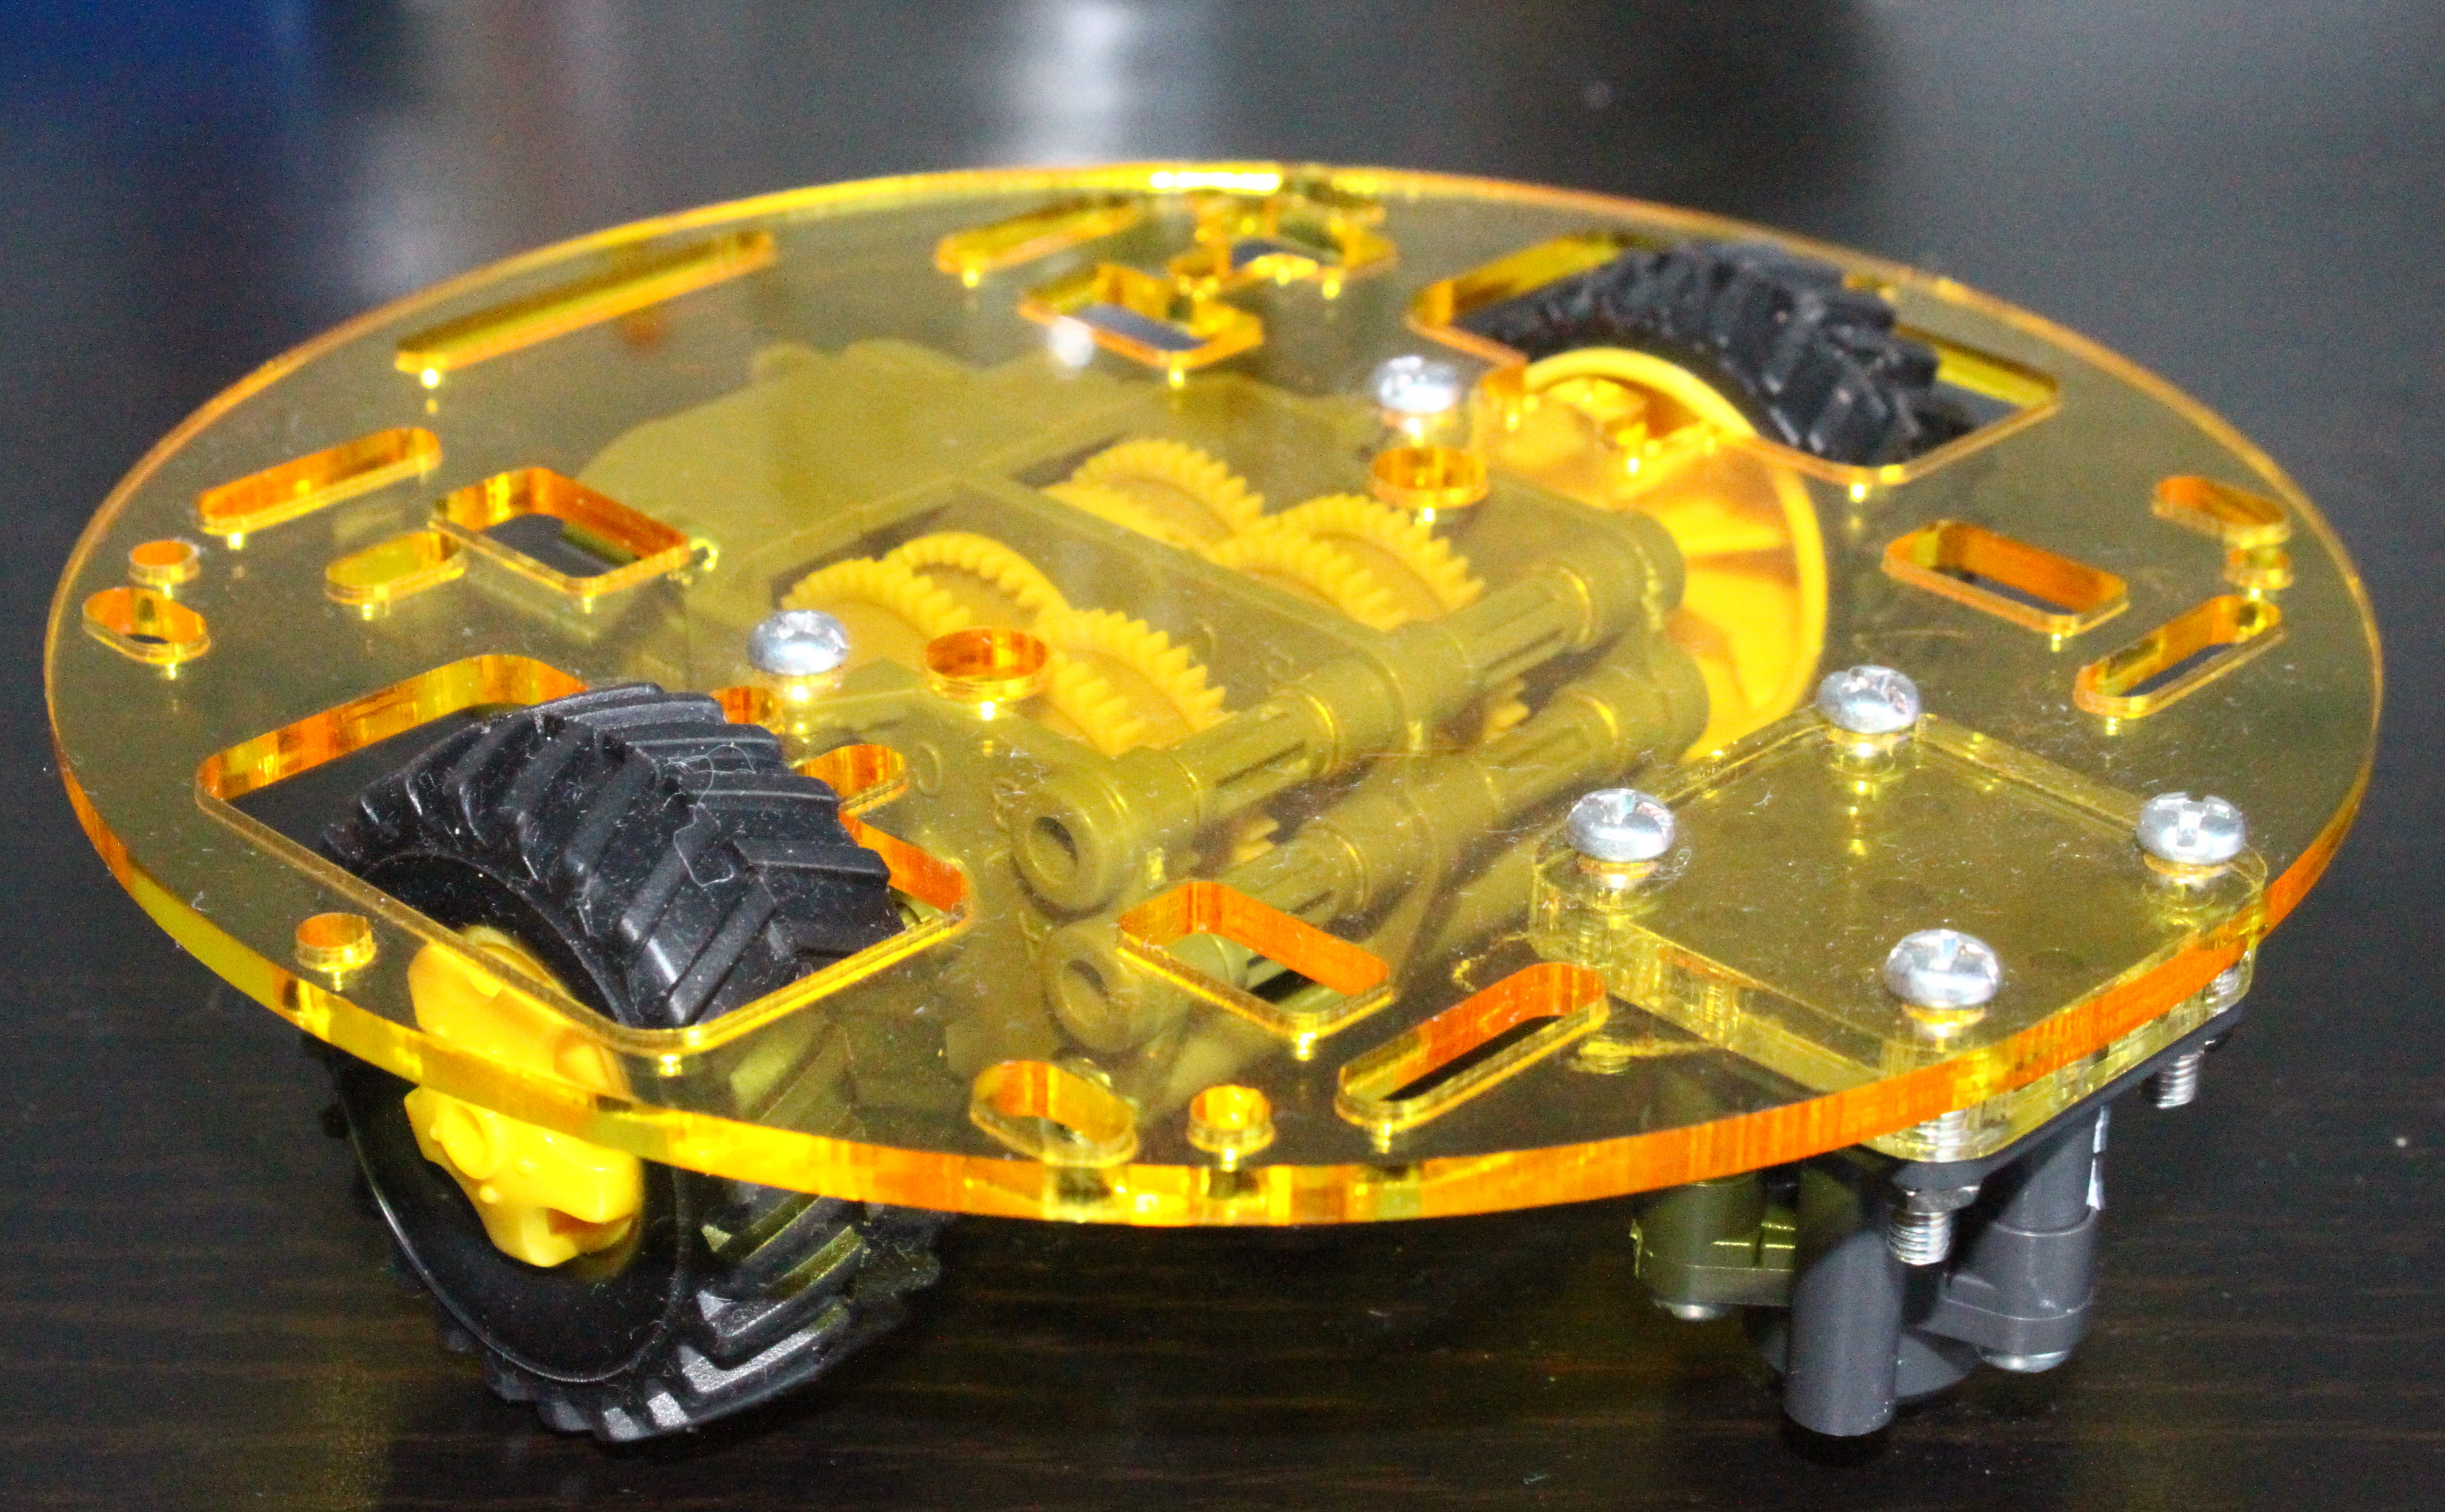
\includegraphics[width=\textwidth]{./Figures/RobotBase.jpg}
\caption{The base of the robot}
\label{fig:RobotBase}
\end{figure}

\section{Project Management}
In order to reduce the risk within the project, all aspects of potential issues are looked at and are summarised in table \ref{tab:risk}. A Gantt chart of how time will be spent can be seen in figure \ref{fig:Gantt}. 

The project will be designed in stages - first, gaining operation of all the basic sections; movement, image capturing, image detection algorithms etc. These will then be brought together once tested to create the final product. 
\begin{table}
\begin{tabular}{|p{6cm}|p{2cm}|p{6cm}|}\hline
Risk						&	Severity	&	Prevention \\ \hline
Parts not arriving on time	&	High		&	Order parts as early as possible \\
Project not fulfilling specification				&	High		&	Develop in stages to obtain functionality in parts. Ensure enough time is allocated to the project.	\\
PCB Design is incorrect		&	Medium		&	Check the design carefully and get second opinion \\
Failure of personal computer causing data loss & Low	& 	Keep back ups of all work on Devtrack Git repository and Dropbox.\\

\hline
\end{tabular}
\caption{A list of risks and the prevention steps taken to reduce their impact}
\label{tab:risk}
\end{table}

%% ----------------------------------------------------------------
%% Research.tex
%% ---------------------------------------------------------------- 
\chapter{Research} \label{Chapter:Research}
The research done for this project is split down into three sections:
\begin{enumerate}
\item Hardware
\item Software, broken down into:
\begin{enumerate}
\item Firmware
\item Algorithms
\end{enumerate}
\end{enumerate}

\section{Hardware Research}
\inote{Talk about why I chose to develop with AVRs, comparison with other uControllers. Why I used the OV7670 Camera etc etc}


\section{Image Algorithms}

\subsection{Comparison Algorithms} 
Before 



%% ----------------------------------------------------------------
%% Hardware Development.tex
%% ---------------------------------------------------------------- 
\chapter{Hardware and Firmware Development} \label{Chapter:HardwareDevelopment}
For initial development, the \textit{Il Matto} board, designed by Steve Gunn, was used. The system has an ATMega644P clocked at 12MHz and has an on-board SD card socket. This provided the ability to prototype circuits which are then used to create a PCB, 

The following section is broken down into the following parts:
\begin{enumerate}
\item[\ref{Section:Camera}] Camera Code
\item[\ref{sect:SDCard}] SD Card
%\item Motor Control
\item[\ref{Section:Motor_Dev}] Motor Development
\item[\ref{Section:PCB_Dev}] PCB Development
\end{enumerate}

\section{Camera} \label{Section:Camera}

The camera used is an OV7670 by OmniVision. It is mounted onto a break out board and connected to a AL422B FIFO Buffer. The breakout board has all passive components needed and a 24MHz clock mounted. The schematic for the device can be seen in appendix \ref{Chapter:AppendixA:CircuitDiagrams}.

Original code for the camera operation was given by Steve Gunn, which was used to gain the operation required. This code streamed continuous video to a TFT screen. The operation required was to take a single photo from the camera and store the data. 

\subsection{Single Camera Operation}

The camera uses a SCCB Interface \citep{SCCB_Interface} created by OmniVision. This is almost identical to the $I^{2}C$ Interface by Phillips and the two protocols are compatible. The original code used a bit-banged SCCB interface which was very slow and used up processing time. This was changed to make used of the built-in interrupt-driven $I^{2}C$ interface (named TWI in Atmel AVRs)\footnote{$I^{2}C$ , SCCB and TWI are all the same but are called differently due to Phillips owning the right to the name ``$I^{2}C$"}. This communication bus is used to set up the control registers of the OV7670 to enable operation in the correct format. 

RGB565 is a 16 bit pixel representation where bits 0:4 represent the blue intensity, 5:10 is the green intensity and 11:15 represent the red intensity (see figure \ref{fig:RGB565}). This is a compact way of storing data but only allows 65536 colours. Greys can also appear to be slightly green due to the inconsistent colour ratio of the green field. This representation was used as it is a compact format to store images in. It is easily converted to grey scale and is a widely used format.
\begin{figure}
\includegraphics[width = \textwidth]{./Figures/RGB565.png}
\caption{RGB565 pixel format}
\label{fig:RGB565}
\end{figure}

The camera must use a high speed clock in order to ensure the pixels obtained are from the same time. This makes it difficult for an AVR to be able to respond to the camera quick enough (ATMegas typically clocked at 8-12MHz). This highlights the necessity for a FIFO Buffer. 

The OV7670 is set up so that the VSYNC pin goes low at the beginning of every full frame of data, and HREF is high when the data being output is valid. The pixel data is then clocked out on every rising edge of PCLK. To control the buffer, WEN (write enable) is NAND with the HREF signal. When both are high, the write enable to the buffer will be active and the data will be clocked in by PCLK. In order to acquire a full frame, the first VSYNC pin is set up to interrupt the AVR to enable WEN. The camera will output an entire frame of pixel data and store it into the buffer. When the second VSYNC is received, the WEN signal is disabled, stopping any more data being stored. At this point, the FIFO buffer contains all the image data.

To obtain the data from the buffer, the AVR sets output enable and pulses the read clock. Valid data is available on the input port while RCLK is high. All the data is then read in half a pixel at a time. The entire operation can be seen in figure \ref{fig:ov_Capture}.
\begin{figure}
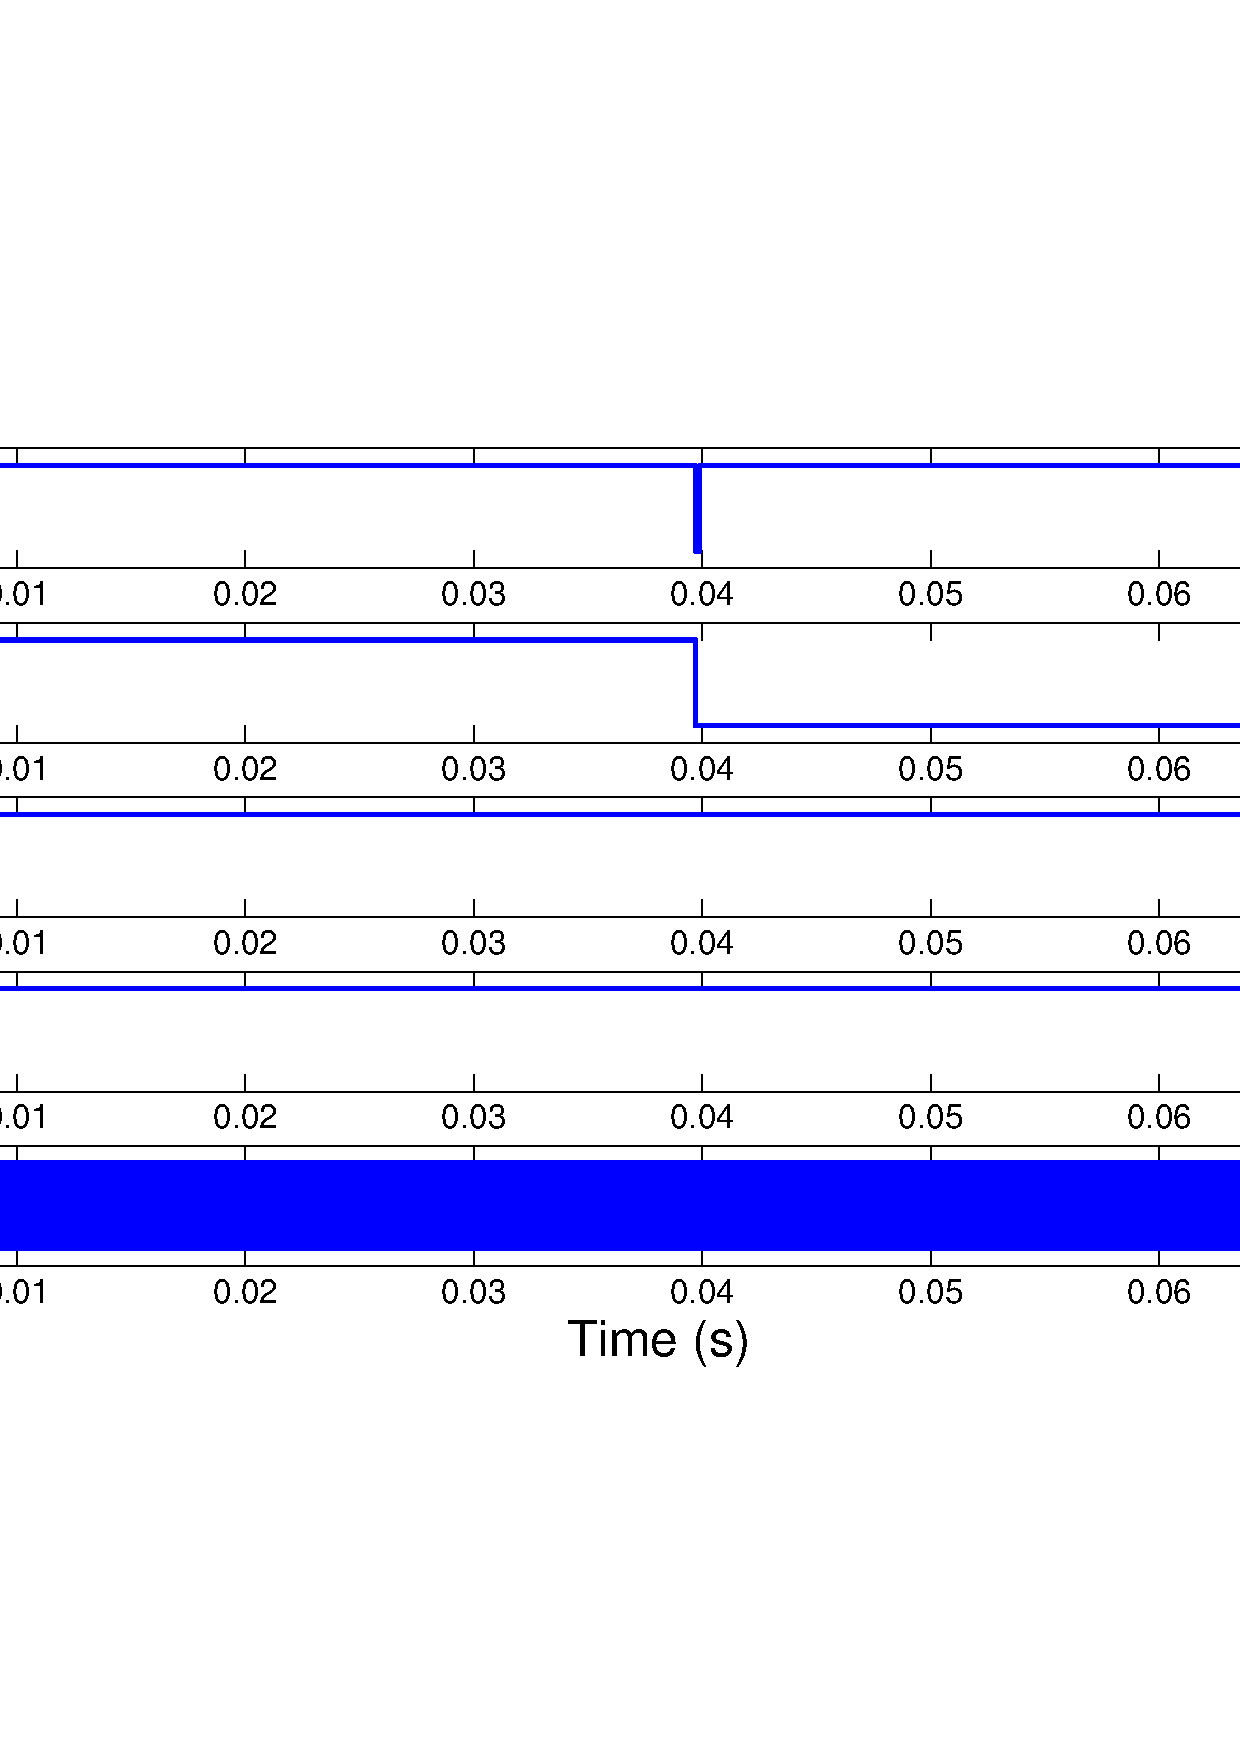
\includegraphics[width = \textwidth]{./Figures/ov7670_im_capture.png}
\caption{Signals generated to control the OV7670 capture and read}
\label{fig:ov_Capture}
\end{figure}


Difficulties arose at this point with the storage of the data. The ATMega644P has 4kB of internal SRAM, but  153.6kB of memory is needed to store a single image at QVGA (320 by 240 pixels, 2 bytes per pixel) quality. 

Firstly, data was sent straight to a desktop computer via a COM Port using USART. A simple desktop program was written in C\# to receive and store all the data, and to make a Bitmap image from the data. This method was slow, taking around 30 seconds to transmit one uncompressed image. 

The second option was to use extra memory connected to the microcontroller. An SD card is used as FAT file system so that data can be looked at by a user on a computer. Text log files are also written to aid debugging. This is discussed in section \ref{sect:SDCard}. 

\subsection{Dual Camera Operation}
In order for stereovision to be successful, two cameras separated by a horizontal distance ($B$) will need to be driven at the same time to obtain photos within a small time frame of one another.

A major problem occurred with using the \itc interface to set up both cameras. The camera has a set \itc address of $21_{16}$, which cannot be changed. Multiple \itc devices with exactly the same address cannot be used on the same bus. 
Two solutions to this are possible: driving one from $I^{2}C$ and one from SCCB, or using an \itc multiplexer. By using two different buses, there can be no bus contention. However, SCCB is slow and processor-hungry as it deals with the protocol bit by bit in software. This takes up memory and is not reusable for other operations.

An \itc multiplexer sits on the bus and has multiple output buses. The master can then address the multiplexer and select whether to pass the bus to bus 0, bus 1 or not allow the data to be transferred. This saves processor time, but means a write operation has to be done to select the camera bus before being able to write to the camera. This slows down the operation, but not as much as using SCCB. The main disadvantage to the \itc MUX is the extra hardware needed; firstly the MUX itself, but also 7 extra resistors to pull up the two extra buses and the three interrupt lines must be added. 

Overall, the disadvantages posed by using a MUX are small, so a multiplexer will be used as opposed to the SCCB interface. A suitable multiplexer is the Phillips PCA9542A \citep{I2C_Mux}.

The buffers have an output enable pin so the data bus can be shared by both cameras to the AVR. The ATMega644P offers three interrupt pins, two of which are used by the two VSYNC pins for the cameras.

Two ISRs are used to control the VSYNC signals, and when taking a photo, both frames are taken at a time period close together to capture the same scenario. The data for both images are read back individually by the AVR. 

Operation to read an image is identical to using one camera. However, an ID number is passed through the functions to make a decision on the pins to use to read the buffer and to enable the output. Care was taken to avoid bus contention, but no checking procedure is explicitly in place. Both images are then read back from the buffers and stored to memory. 

\section{SD Card} \label{sect:SDCard}

To use the SD card, the FATFS library \citep{FATFS} was used. The library supplies all the functions for writing a FAT File System in the files \textit{ff.c}, \textit{ff.h}, \textit{ffconf.h}, \textit{diskio.c}, \textit{diskio.h} and \textit{integer.h}. The \textit{diskio.h} functions control what device is being used - SD/MMC Card, USB drive etc. The \textit{ff.h} header contains all the functions to write to in a FAT File system. 
\\
An SD card was chosen due to it's small size, low cost and a large data storage. The cards work using an SPI bus which can be used for other devices within the system so the card only uses one extra enable pin in hardware to function. 

\subsection{Storing Images}

Many image formats are common, such as Joint Photographic Expert Group (JPEG), Portable Network Graphics (PNG), Bitmap (BMP) and Graphics Interchange Format (GIF). Table \ref{ImageFormats} shows a summary of some common image formats.


\begin{table}
\centering
\begin{tabular}{|p{3cm}| p{2cm}|p{2cm}|p{2cm}|p{2cm}|} \hline
			&	Bitmap 		& 	JPEG			 	&	PNG				& 	GIF \\ \hline
Extension 		& 	*.bmp 		&  	*.jpg /*.jpeg 		& 	*.png				& 	*.gif \\ \hline
Compression 	& 	No 			& 	Lossless  and Lossy		&	Lossless ZIP			&	Lossy	\\\hline
File Size of 320 by 
240 pixel Image (kB) &	225			&	20				&	23				&	24 \\\hline
Bits per Pixel		&	8, 16, 24 or 32	&	24				&	24, 32 or 48 			& 	24, but only 256 Colours \\


\hline
\end{tabular}
\caption{A table comparing different image formats available (\cite{ImageComparison})}
\label{ImageFormats}
\end{table}

It is clear that the best choice for images would be either PNG or JPEG. However, these require more computational time to compress the image into the correct format. To avoid compression, and thereby save processing time, bitmap was chosen at the expense of using more memory. The data in a bitmap image is also stored in RGB format so can be read back easily when processing the image. Appendix \ref{Chapter:AppendixB:BMPFile} shows the make up of a Bitmap File that was used.

By writing the image in this format, they are then able to be opened on any operating system. This aids debugging and allows the prototyping of image algorithms in a more powerful environment. Figure \ref{ExampleImage} shows a photo taken by the OV7670 and stored on a SD card.

\begin{figure}
\begin{center}
\includegraphics{Figures/ExampleImageFromCamera.jpg} 
\end{center}
\caption{An Example Image taken using the OV7670 and stored as a Bitmap on the SD Card}
\label{ExampleImage}
\end{figure}

\subsection{User Interface}
The ATMega 664P pinout for the dual camera operation can be seen in table \ref{table:644Pin}. Due to a lack of available GPIO pins, an ATMega168 was added on the \itc bus to act as a port extender. The ATMega168 accepts a read or write command. A write places the written data on Port D and a read returns any button pressed that occurred on Port C. When a button is pressed, this is stored in the ATMega168 until a read has been done. This is so the master (644P) does not miss any button presses while busy doing lengthy operations such as writing an image. The code is based on Application Note AVVR311 \citep{Atmel:I2CSlave}, written for IAR Compiler. This code was altered to compile with GCC under Atmel Studio. AVRs contain a hardware based \itc protocol that is interrupt based in software. The interrupt service routine of the TWI vector is a state machine which loads the data to send, stores received data, responds to acknowledges and address calls and deals with bus errors that can occur.

\begin{table}
\centering
\begin{tabular}{|c|c|c|c|c|}\hline
	& 	Port A 	& 	Port B 			& 	Port C 				& 	Port D 		\\ \hline
0	&	Data 0	&	SD Write Protect&	\itc - SCL			&	No Connection	\\
1	&	Data 1	&	SD Card Detect	&	\itc - SDA			&	No Connection	\\
2	&	Data 2	&	USB Data Plus	&	Read Clock 1		&	VSync 0			\\
3	&	Data 3	&	USB Data Minus	&	Read Reset 1		&	VSync 1			\\
4	&	Data 4	&	SPI Chip Select	&	Write Enable 1		&	Read Clock 0	\\
5	&	Data 5	&	SPI	MOSI 		&	Write Reset 1		&	Read Reset 0	\\
6	&	Data 6	&	SPI MISO		&	Output Enable 0		&	Write Enable 0	\\
7	&	Data 7	&	SPI Clock		&	Output Enable 1		&	Write Reset 0	\\
\hline

\end{tabular}
\caption{Pin Connections of the ATMega644P for Dual Camera Operation.}
\label{table:644Pin}
\end{table}

The entire prototype for the dual camera operation can be seen in figure \ref{fig:Prototype}. This circuit was developed to test the cameras and is used to develop the PCB in section \ref{Section:PCB_Dev}. 
%\section{Motor Control}
%\inote{do something of this SOON}
%\section{Circuit Development} \label{Section:Circuit_Dev}
%\subsection{Stereo Camera Development}
%Figure \ref{sch:DualCam_Schematic} shows the circuit diagram for the prototype. This uses the Il Matto development board for the main microcontroller. The prototype can be seen in figure \ref{fig:Prototype}. This circuit captured and stored two images from the cameras to the SD card. 
\begin{figure}
\includegraphics[width=\textwidth]{./Figures/Prototype.jpg}
\caption{Prototype of Dual Camera operation.}
\label{fig:Prototype}
\end{figure}
\section{Motor Driver Development}\label{Section:Motor_Dev}
%\inote{Tachometers}
%\inote{Derivation of equations used - Distance / Rotating}

\subsection{Hardware}
Tachometers are devices used to measure rotational speed of a shaft. Tachometers are commonly found in bicycles where a small magnet is attached to the wheel and a sensor is attached to the frame. The elapsed time between every rotation detected by the sensor is measured and, by knowing the size of the wheel, speed can be calculated. 
\inote{Cite Needed}

Here an optosensor, the TCRT1010 made by \cite{Vishay:TCRT1010:Datasheet}, is used to measure rotations of the wheel and used to be able to move a distance determined by the microcontroller. The TCRT1010 package contains an IR LED and a phototransistor. The schematic of a simple transistor amplifier used can be seen in figure \ref{Circuit:TCRT1010} and was taken from \cite{NEEDED}. 
\inote{Cite Needed}

A similar method to the way a bike measures speed was used. The wheel's rubber absorbed the IR, so a high voltage was always seen at the collector of the phototransistor. White tippex marks, ``tabs'', were applied to the wheels at regular intervals. These tabs reflected IR, resulting in a lower collector voltage and thereby giving a way to detect wheel rotation, but not direction. Figure \ref{Graph:WheelVoltage} shows the voltage at the collector (read by the ADC on the AVR) against the angle of the wheel. Ten tabs were marked on the wheel, and ten dips in the voltage can be seen in figure \ref{Graph:WheelVoltage}. 

\inote{Redo this graph!}

\begin{figure}
\centering
\includegraphics[scale=0.5]{Figures/TCRT_Circuit.png}
\caption{Circuit diagram of Optosensor}
\label{Circuit:TCRT1010}
\end{figure}

\begin{figure}
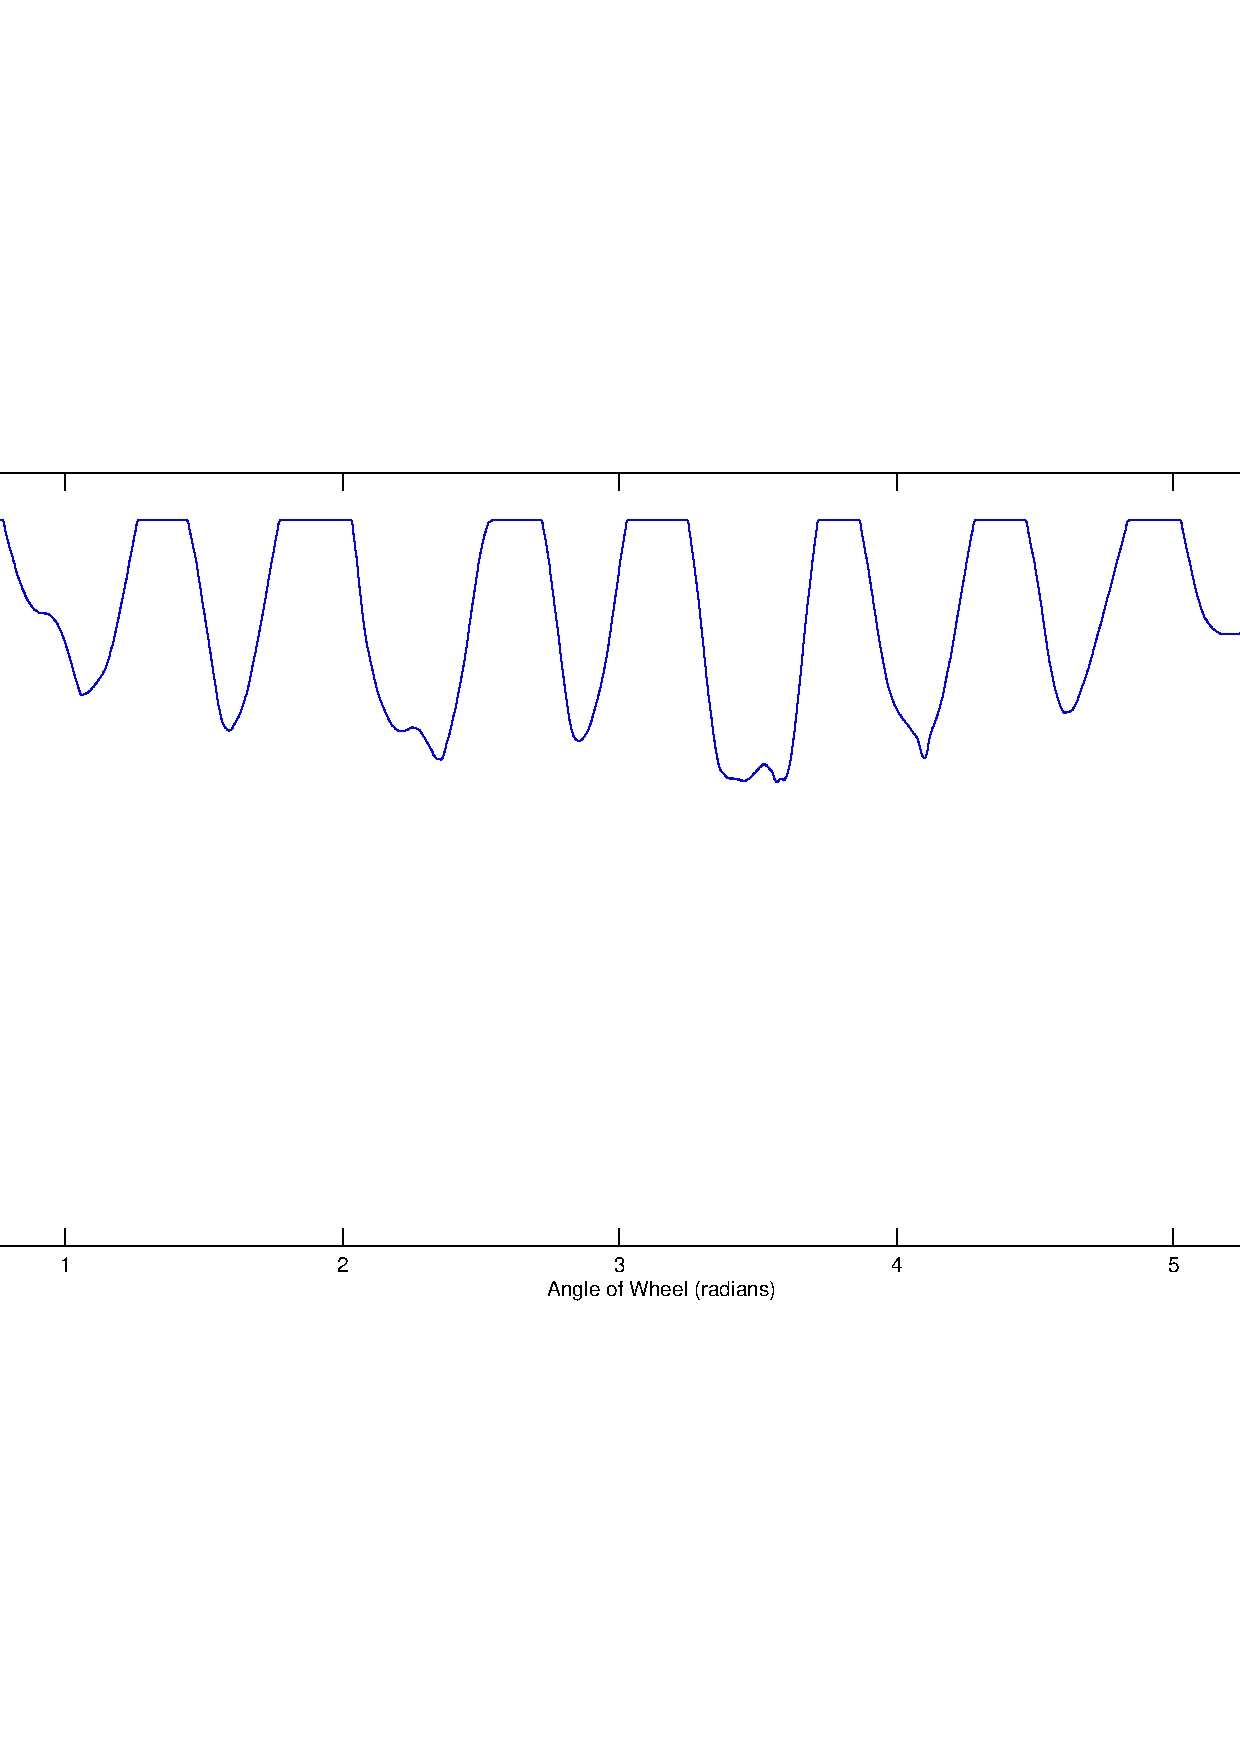
\includegraphics[width = \textwidth]{Figures/WheelVoltageGraph.jpg}
\caption{Graph of Wheel Angle against the Voltage read by the AVR}
\label{Graph:WheelVoltage}
\end{figure}
 

\subsection{Firmware Development}

The basic outline of the firmware is a set up to calculate how many counts are needed to move the distance, set the inputs to the motor drivers and use PWM to control the speed. The number of times the tabs pass the sensor are counted and when the count reaches the correct number, the motors are stopped. The robot can move in either a straight line or rotate on the spot. More complex movements, for example arcs, would require more accurate tachometers and are not discussed here. 

Moving in a straight line takes a parameter of how far to move as a signed integer and calculates the total number of counts that need to occur. This can be calculated using equation \eqref{eq:NumberCounts}. This value is put in a global variable so that other methods have scope to it. 

\begin{equation}
\label{eq:NumberCounts}
\text{Counts} = D \times \frac{\gamma}{C_w}
\end{equation}

For rotation, the radius from the centre of the robot to the wheels needs to be known, see figure \ref{fg:RobotBase:Top}. The circumference through the wheels is then easily calculated and the angle of rotation is then a ratio. The distance to move is calculated by equation \eqref{eq:RotationalDistance} and the total number of interrupts can be calculated using equation \eqref{eq:NumberCounts}. To rotate clockwise, the left motor is driven forward and the right is driven backwards. To rotate anti-clockwise, the directions are reversed.

\begin{equation}
\label{eq:RotationalDistance}
D_{R} = A \times \frac{C_b}{360}
\end{equation}

Combining equations \eqref{eq:NumberCounts} and \eqref{eq:RotationalDistance} gives:
\begin{equation}
\label{eq:RotationalInterrupts}
Interrupts = A \times \frac{\gamma}{C_w} \times \frac{C_b}{360}
\end{equation}
Where $A$ is the angle to rotate in degrees, $\gamma$ is the counts per revolution of the wheel, $C_w$ is the circumference of the wheel and $C_b = 2\pi\times r_b$ and $r_b$ is the distance from the centre of the robot to the centre of the wheel (see figure \ref{fig:RobotBase_Annotated}).


As the voltage swing on the collector of the phototransistor does not reach near 0V, the AVR cannot detect this as a logical 0. An external amplifier could be used to generate a full swing voltage. However, the AVR has ADCs and analogue comparators. 

The ADC could be used to continually sample the collector voltage and detect dips in the signal. This method has the advantage of a variable threshold and the ability to filter noise. The operation, however, would be complex to implement in code. 

An alternative is to use an analogue comparator. The UC3C has two on chip comparator interfaces, each with two comparators. They are a high gain Op Amp with added options for hysteresis and the ability to interrupt amongst other attributes. The comparators can use two analogue inputs or use the internal DACs as inputs. Potentiometers were used to set the reference voltage externally. %but this was later changed to use the internal DAC to reduce power consumption. Using the DAC means the microcontroller can have dynamic control over the threshold. 
This method has the advantage of returning a boolean value of if the collector voltage is higher or lower than the threshold voltage. The detection is easier to detect than reading ADC values and the code will be simpler to implement. This method was decided on for an easier implementation.

The first method implemented was to use the analogue comparators to interrupt when the collector voltage crossed the threshold. Both wheels used the same comparator interface and therefore ran the same ISR when triggered. The ISR then had to read the output of the comparators and decrement the relevant counter for the correct wheel. This method had many downfalls. First, it was not possible to know which comparator caused the interrupt. If the left wheel triggered the interrupt while the right was below the threshold, both left and right counters would be decremented. This caused a large error each time it occurred. Another problem was noise; occasionally, the lowering voltage would cause multiple interrupts each time. This problem was reduced by setting the hysteresis on the comparators but did not solve the problem completely. 

A second approach utilised a simple state machine and software based hysteresis to solve the problems. After the set up is complete, the method \textit{Motors\_Execute} is run, containing the state machine to control the motors. The state machine has two states `On a Tab' and `Not on a Tab'. When the method enters, the initial state is read from the comparators. If the wheel is already on a tab, it won't be counted. The code then runs in a loop until the motors stop. A graphic representation of the code can be seen in figure \ref{fig:StateMachine}. Starting in `Not on a Tab' state, a tab must be detected for Hyst\_Max cycles in succession for the state to change. This is the same for going from `On a Tab' to `Not on a Tab'. This is to reduce noise in the form of false readings an increase the certainty that a tab is in detect. The Global\_Count is only reduced on the transition to `On a Tab' so it is difficult for this to decrement multiple times in normal operation. To increase the certainty, Hyst\_Max can be increased at the expense of response time. 


\begin{figure}
\includegraphics[width=\textwidth]{Figures/ASM.jpg}
\caption{A State Machine showing the operation of the \textit{Motor\_Execute} method}
\label{fig:StateMachine}
\end{figure}


\begin{figure}
\centering
\subfigure[Top View of robot base showing dimensions of interest\label{fg:RobotBase:Top}]{\includegraphics[width = \textwidth, keepaspectratio]{./Figures/Robotbase_top_annot.jpg} }
\subfigure[Side View of robot base showing dimensions of interest\label{fg:RobotBase:Side}]{\includegraphics[width = \textwidth, keepaspectratio]{./Figures/Robotbase_side_annot.jpg} }
\caption{Dimensions of Interest for Robot Movement}
\label{fig:RobotBase_Annotated}
\end{figure}

The motor speed was controlled by PWM. The code sets up a low duty cycle PWM signal to drive the motors slowly. This causes any overshoot that could happen to be low and removes the need for a speed controller. 

The final code can be seen in appendix \ref{Chapter:AppendixC:Code}


\subsection{Testing}\label{Section:MotorTest}
\inote{Test Rotation}

To test the motor system, different distances were given to the movement method. The method prints how many counts will be moved. The actual distance moved was then measured and repeated four times. Table \ref{table:results:motor:distance} shows the results of this test and figure \ref{fig:results:motor:distance}. The results show that the maximum error observed is $4.52\%$, which related to $4.5mm$. This error is acceptable as a half centimetre error over 10 will not impact the performance of the robot. 


\begin{table}
\caption{Results of Motor Distance Test}
\label{table:results:motor:distance}
\begin{tabular}{|p{2.5cm}|p{2.5cm}|p{2.5cm}|p{2.5cm}|p{2.5cm}|} \hline
Distance Specified (mm) &	Number of Counts Returned	& 	Counts $\times$ Resolution (mm)	& 	Average Measured Distance Moved (mm)	&	Error (\%) \\ \hline
50						&	4							&	46.4							&	47.25									&	1.83		\\
75						&	6							&	69.6							&	70.75									&	1.65		\\
100						&	8							&	92.8							&	97.0									&	4.52		\\
120						&	10							&	116.0							&	113.25									&	2.37		\\
150						&	12							&	139.2							&	141.0									&	1.29		\\
170						&	14							&	162.4							&	161.5									&	0.55		\\
200						&	17							&	197.2							&	201.5									&	2.18		\\
250						&	21							&	243.6							&	244.5									&	0.37		\\
300						&	25							&	290.0							&	290.75									&	0.26		\\ \hline
\end{tabular}
\end{table}

\begin{figure}
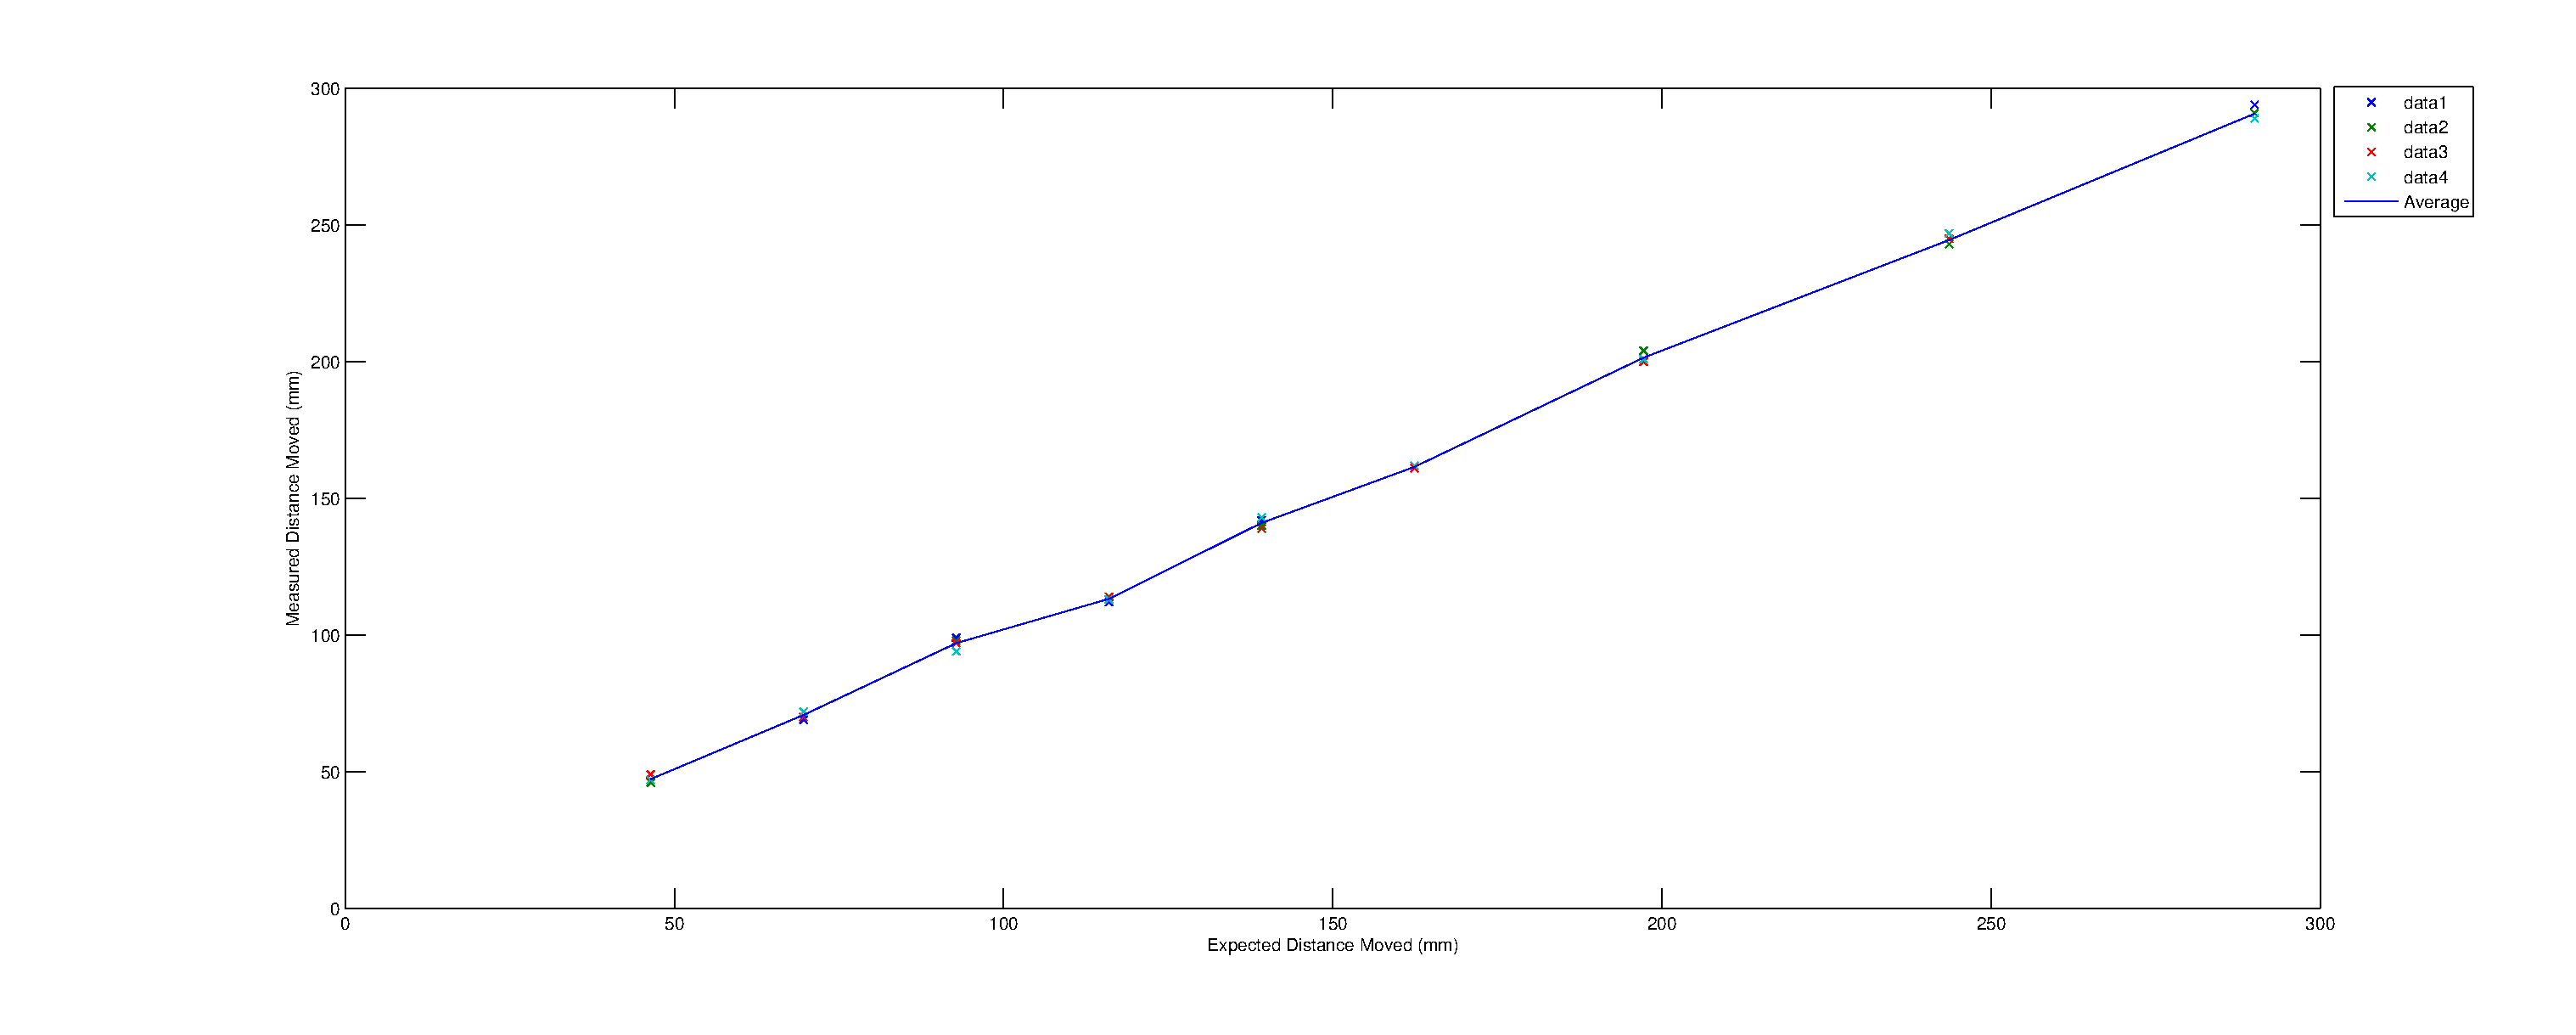
\includegraphics[width=\textwidth]{Figures/Motor_Distance.eps}
\caption{A plot of Expected Distance against the measured data. Line indicates the average of the data at each point.}
\label{fig:results:motor:distance}
\end{figure}

A problem was seen that the robot moved in a slight arc. Speed tests were done on the wheel by measuring the total time taken to complete eight full revolutions, the equivalent of moving 928mm. The results and the calculated wheel speeds can be seen in table \ref{table:results:motor:speed}. It shows that the left motor runs slightly faster than the right, even though the PWM duty cycle is the same. A proportional controller could be implemented to correct this error during operation. However, over the distances covered, the error introduced by this is small enough to neglect. 

\begin{table}
\caption{Results of motor speed test}
\label{table:results:motor:speed}
\centering
\begin{tabular}{|c|c|c|} \hline
Wheel &	Total Time Elapsed ($s$) & Calculated Speed ($mm.s^{-1}$) \\ \hline
Left & 44.6		&	20.8 \\ \hline
Right & 49.6	&	18.7 \\ \hline
\end{tabular}
\end{table}

\subsection{Conclusion}
Due to the low resolution of the sensor (10 counts per revolution), there is a minimum distance that can be moved and a minimum angle of rotation, shown in equations \eqref{eq:Resolution:Distance} and \eqref{eq:Resolution:Angle} respectively. These show that greater distance resolution can be obtained by decreasing the wheel size or increasing $\gamma$ and a greater rotational resolution can be obtained by the same as distance, or by increasing the distance the wheels are from the centre of the robot. 


\begin{equation}\label{eq:Resolution:Distance}
\Delta_{d} = \frac{C_w}{\gamma} = 12mm
\end{equation}
\begin{equation}\label{eq:Resolution:Angle}
\Delta_{\theta} = \frac{360 \times C_w}{\gamma \times C_b} \approx 15^\circ 
\end{equation}

This method lacks on two points - lack of speed control and accuracy.
A better controller could be implemented to help move at different speeds. This could use the remaining number of counts to gradually slow the speed of the motors down proportionally as well as correct the speed mismatch between the wheels. A PID controller could be implemented if greater accuracy is needed quicker, at the expense of computation time and potential overshoot. 

Rotary encoders could be used to detect the direction of wheels as well. A good, but more costly, alternative would be the HUB-ee wheel by \cite{Creative_Robotics}, which includes a 120 point quadrature encoder and sensor, motor driver and a geared motor all within the wheel. These wheels have 12 times the accuracy as the method described here and a similar interface. 
 
Given that the robot does not need to move any more accurately that to 1cm, this method has proved to be cheap and successful. The robot is able to move a distance with reasonable accuracy, but to a fairly low resolution.

\section{PCB Development}\label{Section:PCB_Dev}
\subsection{Circuit Design}

Figure \ref{fig:Hierarchical} shows a basic hierarchy of the robot. Each pin on the AT32UC3C0512C can have one of six special functions, as well as being a GPIO pin.  Table \ref{table:UC3C:Pinout} shows the pinout for the microcontroller used. 
\begin{figure}
\includegraphics[width=\textwidth]{Figures/hierarchy.jpg}
\caption{A Hierarchical diagram of the robot}
\label{fig:Hierarchical}
\end{figure}

\begin{table}
\caption{The Pinout of the AVR for the circuit. '-' means unavailable and blank means unused}
\label{table:UC3C:Pinout}
\begin{tabular}{|c|c|c|c|c|}\cline{2-5}
\multicolumn{1}{c|}{ } & \multicolumn{4}{|c|}{Port} \\ \hline
Pin & A & B & C & D \\ \hline
0&TCK&CAMERA\_ 0&&EBI-DATA13\\
1&TDI&CAMERA\_ 1&&EBI-DATA14\\
2&TDO&CAMERA\_2&SDA&EBI-DATA15\\
3&TMS&CAMERA\_3&SCL&EBI-ADDR0\\
4&USB ID&CAMERA\_4&USART TXD&EBI-ADDR1\\
5&&CAMERA\_5&USART RXD&EBI-ADDR2\\
6&AC R&CAMERA\_6&&EBI-ADDR3\\
7&AC R&CAMERA\_7&EBI NCS3&EBI-ADDR4\\
8&AC L&STBY1&EBI NCS0&EBI-ADDR5\\
9&AC L&IN11&EBI-ADDR23&EBI-ADDR6\\
10&VSYNC0&IN12&EBI-ADDR22&EBI-ADDR7\\
11&ADCREF&PWM1&EBI-ADDR21&EBI-ADDR8\\
12&&&EBI-ADDR20&EBI-ADDR9\\
13&&PWM2&&EBI-SDCK\\
14&&IN22&EBI-SDCKE&EBI-ADDR10\\
15&RRST0&IN21&EBI-SDWE&EBI-ADDR11\\
16&ADCREF&STBY2&EBI-CAS&EBI-ADDR12\\
17&-&&EBI-RAS&EBI-ADDR13\\
18&-&&EBI-SDA10&EBI-ADDR14\\
19&RCLK0&SPI-MOSI&EBI-DATA0&EBI-ADDR15\\
20&WEN0&SPI-MISO&EBI-DATA1&EBI-ADDR16\\
21&WRST0&SPI-SCK&EBI-DATA2&EBI-ADDR17\\
22&RRST1&SPI-CS3&EBI-DATA3&EBI-ADDR18\\
23&RCLK1&SPI-CS2&EBI-DATA4&EBI-ADDR19\\
24&WEN1&SPI-CS1&EBI-DATA5&EBI-NWE1\\
25&WRST1&SPI-CS0&EBI-DATA6&EBI-NWE0\\
26&VSYNC1&SD- DETECT&EBI-DATA7&EBI-NRD\\
27&NOE1&&EBI-DATA8&EBI NCS1\\
28&NOE0&&EBI-DATA9&EBI NCS2\\
29&&&EBI-DATA10&\\
30&-&CLK&EBI-DATA11&EBI-NWAIT\\
31&-&CLK&EBI-DATA12&-\\ \hline

\end{tabular}
\end{table}

The circuit diagram for Revision A can be seen in section \ref{sch:Columbus:CircuitDiagram}. The schematic for the SDRAM and values and locations of decoupling capacitors were used from the schematic of the UC3C-EK development board \citep{Atmel:UC3CEK}. 
\subsection{PCB Design}
The PCB was designed using EAGLE CAD Software. A four layer board was decided to be used to reduce the number of tracks and more easily supply power and ground to the devices. Layer two is a 3V3 plane and layer three is a ground plane. A ground plane is also on the top and bottom layers to help eliminate any ground bounce that could occur. 

The SDRAM uses the EBI protocol. In high speed systems, care is often taken to equalise track lengths \citep{liu2004equalization}. The UC3C maximum clock frequency is 33MHz (with no wait states), which is not fast enough to cause any track equalisation problems. Care, however, was taken on the USB lines to ensure correct impedance and the tracks lengths matched to each other.

Tracks were routed in order of priority, starting with the UC3C, SDRAM and cameras. All other devices were then routed (\itc MUX, SD card, motor drivers etc). As a precaution, spare pins from the UC3C were routed to a header (J8 and J9) so that additions could be done if a pinout or connection was found to be incorrect. UART, \itc and SPI connections were routed to headers J7, J4 and J5 respectively so logic analysers and COM Port could be attached easily for debugging, or so that extra devices could be added onto the respective protocols. 

%Most of the passives used were 0603 size, but some 1206 capactitors were used for decoupling the voltage regulator and a 1206 diode was used for the analogue reference circuitry. LEDs were also 1206 size. All headers were 0.1'' spaced and a mini B USB socket was used. 
Passives used were all surface mount of either 0603 or 1206 size to save space on the board. All headers used were 0.1'' spaced for easy connections and a mini B USB socket was added for either power or so that the robot can act as a USB device. 

The layout of components was important. The cameras needed to be as far apart as possible and at the front of the PCB. The motor drivers were situated toward the back of the PCB and headers were added to connect the motors to. The optosensors were positioned such that they could be mounted directly on the PCB and be in the correct position to sense the wheels. Mounting holes were also added onto the board so the PCB could be mounted on to the robot base easily. The overall dimensions of the PCB were $100mm \times 70mm$. A full list of components and cost of each is documented in Appendix \ref{Appendix:Costings}


Finally, the name ``The Columbus'' was decided on as the original application for the project was a mapping robot that would search out an unknown area, so the robot was named after Christopher Columbus who explored and navigated parts of the American continents which were unknown at the time. The Eagle CAD Diagram of the PCB can be seen in Appendix \ref{Appendix:PCB}. The PCB was manufactured by \cite{PCBCart}. The PCB cost \pounds 205 to manufacture and ship. A photo of the PCB can be seen in figure \ref{fig:PCB:Bare}. 

\begin{figure}
\includegraphics[width=\textwidth]{./Figures/PCB_Bare.jpg}
\caption{PCB with no components. Left: Top View. Right: Bottom View}
\label{fig:PCB:Bare}
\end{figure}

\inote{Considerations - Power consumption of devices not exceeding VReg}

\subsection{PCB Testing}
A program was written to test all the devices on the PCB. The following tests are done:
\begin{enumerate}
\item UART Send and Receive
\item SD Card Test
\item All LEDs on and off
\item SDRAM Test
\item \itc Test
\item Camera Test
\item Motor Test
\end{enumerate}
The folowing sections explain the tests done to check the devices and protocols worked.

\subsubsection{UART Test}
When the test program begins, the microcontroller waits for a character input. All characters are echoed back. This enables the user to check the communications work. Once a carriage return key is received ($13_{10}$), the test program continues. Listing \ref{lst:UARTTestCode} shows the test code for the UART protocol.

\lstinputlisting[style=C,caption=UART Test Code,label={lst:UARTTestCode},frame=single,numbers=left,tabsize=2,breaklines=true, firstline=110,lastline=121]{../Code/ColumbusTest/ColumbusTest/src/main.c}


\subsubsection{SD Card Test}
The Atmel Software Framework \citep{Atmel:ASF} provided drivers and code for SPI communications and use of a FAT32 File System. The code was configured to use the correct Chip Select pin for the SD Card and the correct SPI Bus was also configured. The test consists of initialising the memory, reading the capacity of the card and printing it to the user. 

The AVR then proceeds to delete any previous log file, create a new log file and writes \textit{``Columbus Tester''} to it. The first 8 characters, which should be \textit{``Columbus''} are read back and checked.
\lstinputlisting[style=C,caption=UART Test Code,label={lst:SDTestCode},frame=single,numbers=left,tabsize=2,breaklines=true, firstline=124,lastline=196]{../Code/ColumbusTest/ColumbusTest/src/main.c}

This exercises all basic File I/O functions, creating, reading and writing and checks them on the device.

\subsubsection{LED Test}
All LEDs are turned on for 1 second, and then turned off. The user should check this occurs. It verifies that all the LEDs are functional and correctly mounted. The Power LED should be on when power is supplied to the PCB. 

\subsubsection{SDRAM Test}
The SDRAM test consists of initialising the SDRAM, calculating the SDRAM Size, writing a unique test pattern to the whole memory, and then reading it back and checking it. The total number of errors are reported. 

The test was adapted from an Example Application from the Atmel Software Framework \citep{Atmel:ASF}. The code can be seen in listing \ref{lst:SDRAMTestCode}. It consists of two \textit{for} loops. In the first, the iteration number is assigned to the memory location. The second loop reads back the data and checks it is correct. An int, \textit{noErrors}, is used to count errors. 

\lstinputlisting[style=C,caption=SDRAM Test Code,label={lst:SDRAMTestCode},frame=single,numbers=left,tabsize=2,breaklines=true, firstline=217,lastline=258]{../Code/ColumbusTest/ColumbusTest/src/main.c}

\subsubsection{\itc Test}
The \itc test checks the bus for devices. It prints out a table showing the address of any devices that acknowledge a probe. A probe is a set up to write to the address. If a device exists on the line, it should Acknowledge \citep{Philips:I2C}. The test is done three times, with no channel selected on the \itc MUX, with channel 0 selected and with channel 1 selected. The two addresses expected at $21_{16}$ for the OV7670 Camera and $74_{16}$ for the \itc MUX. The camera should only acknowledge when the \itc MUX has the relevant channel selected. Listing \ref{lst:TWITestCode} shows the test code for the \itc bus and listing \ref{lst:TWITestCode} shows the result from the full bus scan with channel 0 selected. The cameras are both checked to exist.
\lstinputlisting[style=C,caption=\itc Test Code,label={lst:TWITestCode},frame=single,numbers=left,tabsize=2,breaklines=true, firstline=268,lastline=315]{../Code/ColumbusTest/ColumbusTest/src/main.c}

\begin{lstlisting}[caption={Result of \itc bus scan with Channel 0 of the \itc MUX selected},label={lst:I2CTest}]
Scanning Channel 0
h 0 1 2 3 4 5 6 7 8 9 A B C D E F
0 - - - - - - - - - - - - - - - -
1 - - - - - - - - - - - - - - - -
2 - A - - - - - - - - - - - - - -
3 - - - - - - - - - - - - - - - -
4 - - - - - - - - - - - - - - - -
5 - - - - - - - - - - - - - - - -
6 - - - - - - - - - - - - - - - -
7 - - - - A - - - - - - - - - - -
\end{lstlisting}

\subsubsection{Camera Test}

This test consists of initialising both cameras and checking it passes. Two photos are then taken and stored to the SD card. Success or Failure is displayed. Two images should exists on the SD card from the two cameras. Listing \ref{lst:CameraTestCode} shows the code to conduct this test.
\lstinputlisting[style=C,caption=Camera Test Code,label={lst:CameraTestCode},frame=single,numbers=left,tabsize=2,breaklines=true, firstline=316,lastline=338]{../Code/ColumbusTest/ColumbusTest/src/main.c}

\subsubsection{Motor Driver Test}
An extensive test of the motor driver is discussed in section \ref{Section:MotorTest}. The test code in this application resets the motors so that they are aligned to a white tab on the wheel. This code can be seen in listing \ref{lst:MotorTestCode}. The robot should move no further than 2cm to reach a white tab and the motors should drive forward. This test is useful here to ensure the motors are connected the correct way around and that the potentiometers are set to an appropriate level.

\lstinputlisting[style=C,caption=Motor Test Code,label={lst:MotorTestCode},frame=single,numbers=left,tabsize=2,breaklines=true, firstline=339,lastline=346]{../Code/ColumbusTest/ColumbusTest/src/main.c}

\subsection{PCB Faults}\inote{TCRT1010 Footprint}
During the build and test of the PCB, a number of faults were found. Each is explained and the solution for the problem given. 
\subsubsection{SDRAM Footprint}
The SDRAM footprint made was done exactly to the specification of the pad size and locations with no consideration for soldering to. This meant the chip fit exactly on to the footprint. This made soldering difficult as pads had to be preloaded with solder and the device's pins were heated and bound to the solder. The chip does not seat flat against the PCB. It also put the device at risk as more heat had to be used that usually necessary. Figure \ref{fig:SDRAM_Err} shows the SDRAM chip against the footprint. There is no extra space on the pad to be able to easily solder the device.

\begin{figure}
\centering
\includegraphics[width=\textwidth / 2]{./Figures/PCB_SDRAM.jpg}
\caption{SDRAM Chip shown against its footprint.}
\label{fig:SDRAM_Err}
\end{figure}

To avoid this, existing footprints could be used from other libraries, or double checking the footprints made. The problem meant extra care during soldering had to be taken but has not impeded the operation of the device. 

\subsubsection{SDRAM Chip Select}
The code was prototyped on the Atmel UC3C-EK development board prior to the PCB arriving. When the PCB was built, the code did not work, even with the Chip Select declaration changed. To diagnose this problem, the control lines of the SDRAM were probed with a logic analyser. On the UC3C-EK, the bus was busy with refresh cycles outside of SDRAM access. On the Columbus, no activity was seen. 

The reason the correct control wasn't being seen was due to the UC3C device having a dedicated SDRAM controller, attached to only Chip Select line 1. The Columbus was designed to used chip select line 0. Chip select 1 was available on an external pin, and a via through the routing was close to a via connected to the SDRAM chip select line. Therefore, to overcome the problem, a small enameled wire was soldered to join the two vias together. This solved the problem and the correct signals were then seen on the control lines. The patch can be seen in figure \ref{fig:PCB:Bottom}. 

This fault was caused by not reading the datasheet carefully and ignoring a proven circuit diagram. 

\subsubsection{SDRAM Data Line Resistors}
Once the chip select problem was solved, data returned was unreliable. The SDRAM is word (32 bit) addressed, but accessed in 16 bits. This means read cycles are done per word read. 
Upon investigation of this problem, the 14th, 15th, 30th and 31st (top two bits of each 16 bit access) seemed to read as a 1 the majority of the time. This result wasn't repeatable and sometimes returned correct data. The other bits of the data were always correct. Table \ref{table:SDRAM_Err} shows some examples of the problematic data bits. The data written should match the data read back. 

\begin{table}[!ht]
\caption{A table showing examples of the incorrect data returned from the SDRAM}
\label{table:SDRAM_Err}
\begin{tabular}{c c}
Data Written							&	Data Read \\
00000000 00000000 00000000 00000000		&	\textcolor{red}{11}000000 00000000 \textcolor{red}{11}000000 00000000 \\
00001111 00001111 00001111 00001111		&	\textcolor{red}{11}001111 00001111 \textcolor{red}{11}001111 00001111 \\
\end{tabular}
\end{table}

The problem was traced to resistors \textbf{R31} and \textbf{R32}. They were soldered on incorrectly so that the two data lines of the SDRAM were connected together and the two AVR GPIO pins were connected together. Data was then read back from, effectively, a high impedance line and therefore varied. Once the resistors were soldered correctly, the issue no longer persisted and the whole SDRAM test passed. By utilising the soldermask more, device orientations could be added to ensure correct placement. This can be extended to other devices, such as diodes and capacitors, especially in densely populated areas. 

\subsubsection{Camera Interrupt Line}

As discussed in section \ref{Section:Camera}, the OV7670 needs an interrupt line to synchronise quickly to the start of the frame and is done by using an interrupt line. The UC3C0512C has 9 external interrupt lines. On the PCB, interrupt lines 0 and 1 were used for this control.

Interrupt line 1 was easily configured and worked as expected. However, interrupt 0 did not seem to trigger the interrupt service routine. It was found that interrupt 0 was a ``Non Maskable Interrupt'' which has specific uses and cannot be used in to trigger a method. 

The external interrupt 4 pin was wired to Junction 8 on the PCB. A wire was attached to the camera's VSYNC line and attached to the relevant pin on the header. The operation was then easily obtained and the VSYNC line triggered correctly.

This issues would have been avoided with more understanding of the device before hand and checking the datasheet.


\subsubsection{Motor Driver Pinout}

An error was made in creating the device for the TB6593FNG Motor Driver in EAGLE. On the device, each motor output has two pins to drive each side of the motor. The pin assignment was mixed up when created and connected the two outputs together. Figure \ref{fig:Motor:Error} shows the track errors on one of the motor drivers. 

\begin{figure}
\centering
\includegraphics[width = \textwidth /2]{./Figures/MotorDriver_error.png}
\caption{Motor Driver error. Outputs incorrectly connected}
\label{fig:Motor:Error}
\end{figure}

To solve this, pins 7 and 14 were lifted and removed so that output 1 and output 2 were not connected together. The devices were not damaged in the process of testing this and the motors functioned correctly after this. Double checking the footprints made against the datasheet would have avoided this problem. No impedance to the operation of the drivers has been seen, but the patch may hinder the devices ability to sink current to the motors. 

\subsection{PCB Conclusions}
A number of faults were made in the PCB design. They are:
\begin{itemize}
\item SDRAM footprint
\item SDRAM chip select line
\item SDRAM data line resistors
\item Camera interrupt line
\item Motor driver pinout
\end{itemize}
Three of the faults could have been avoided by consulting the datasheet more carefully during the circuit design stage. The footprint error was due to not being experienced in designing footprints and the data line resistors was a mistake due to lack of attention being paid. 

For future PCBs, more care will be taken in circuit design, with prototyping of circuits with the hardware that will be used. This will highlight any pin specific operations (e.g. the non maskable interrupt) and reduce debugging post production. The effectiveness of a soldermask is also apparent, so more time spent on utilising this would be helpful during assembly.

The PCB itself, was a success. It was a complex PCB with many potential things that could have gone wrong. It was the first PCB I had designed and was a four layer board, using some devices that I did not have experience with. All devices are functional (with a few small modifications) on the PCB so firmware development could continue with all hardware able to be used.


\inote{Redo Bottom of PCB Photo}
\begin{figure}
\centering
\subfigure[Top view of built PCB\label{fig:PCB:Top}]{\includegraphics[width = \textwidth, keepaspectratio]{./Figures/PCB_Top.jpg} }
\subfigure[Bottom view of built PCB with SDRAM chip select patch \label{fig:PCB:Bottom}]{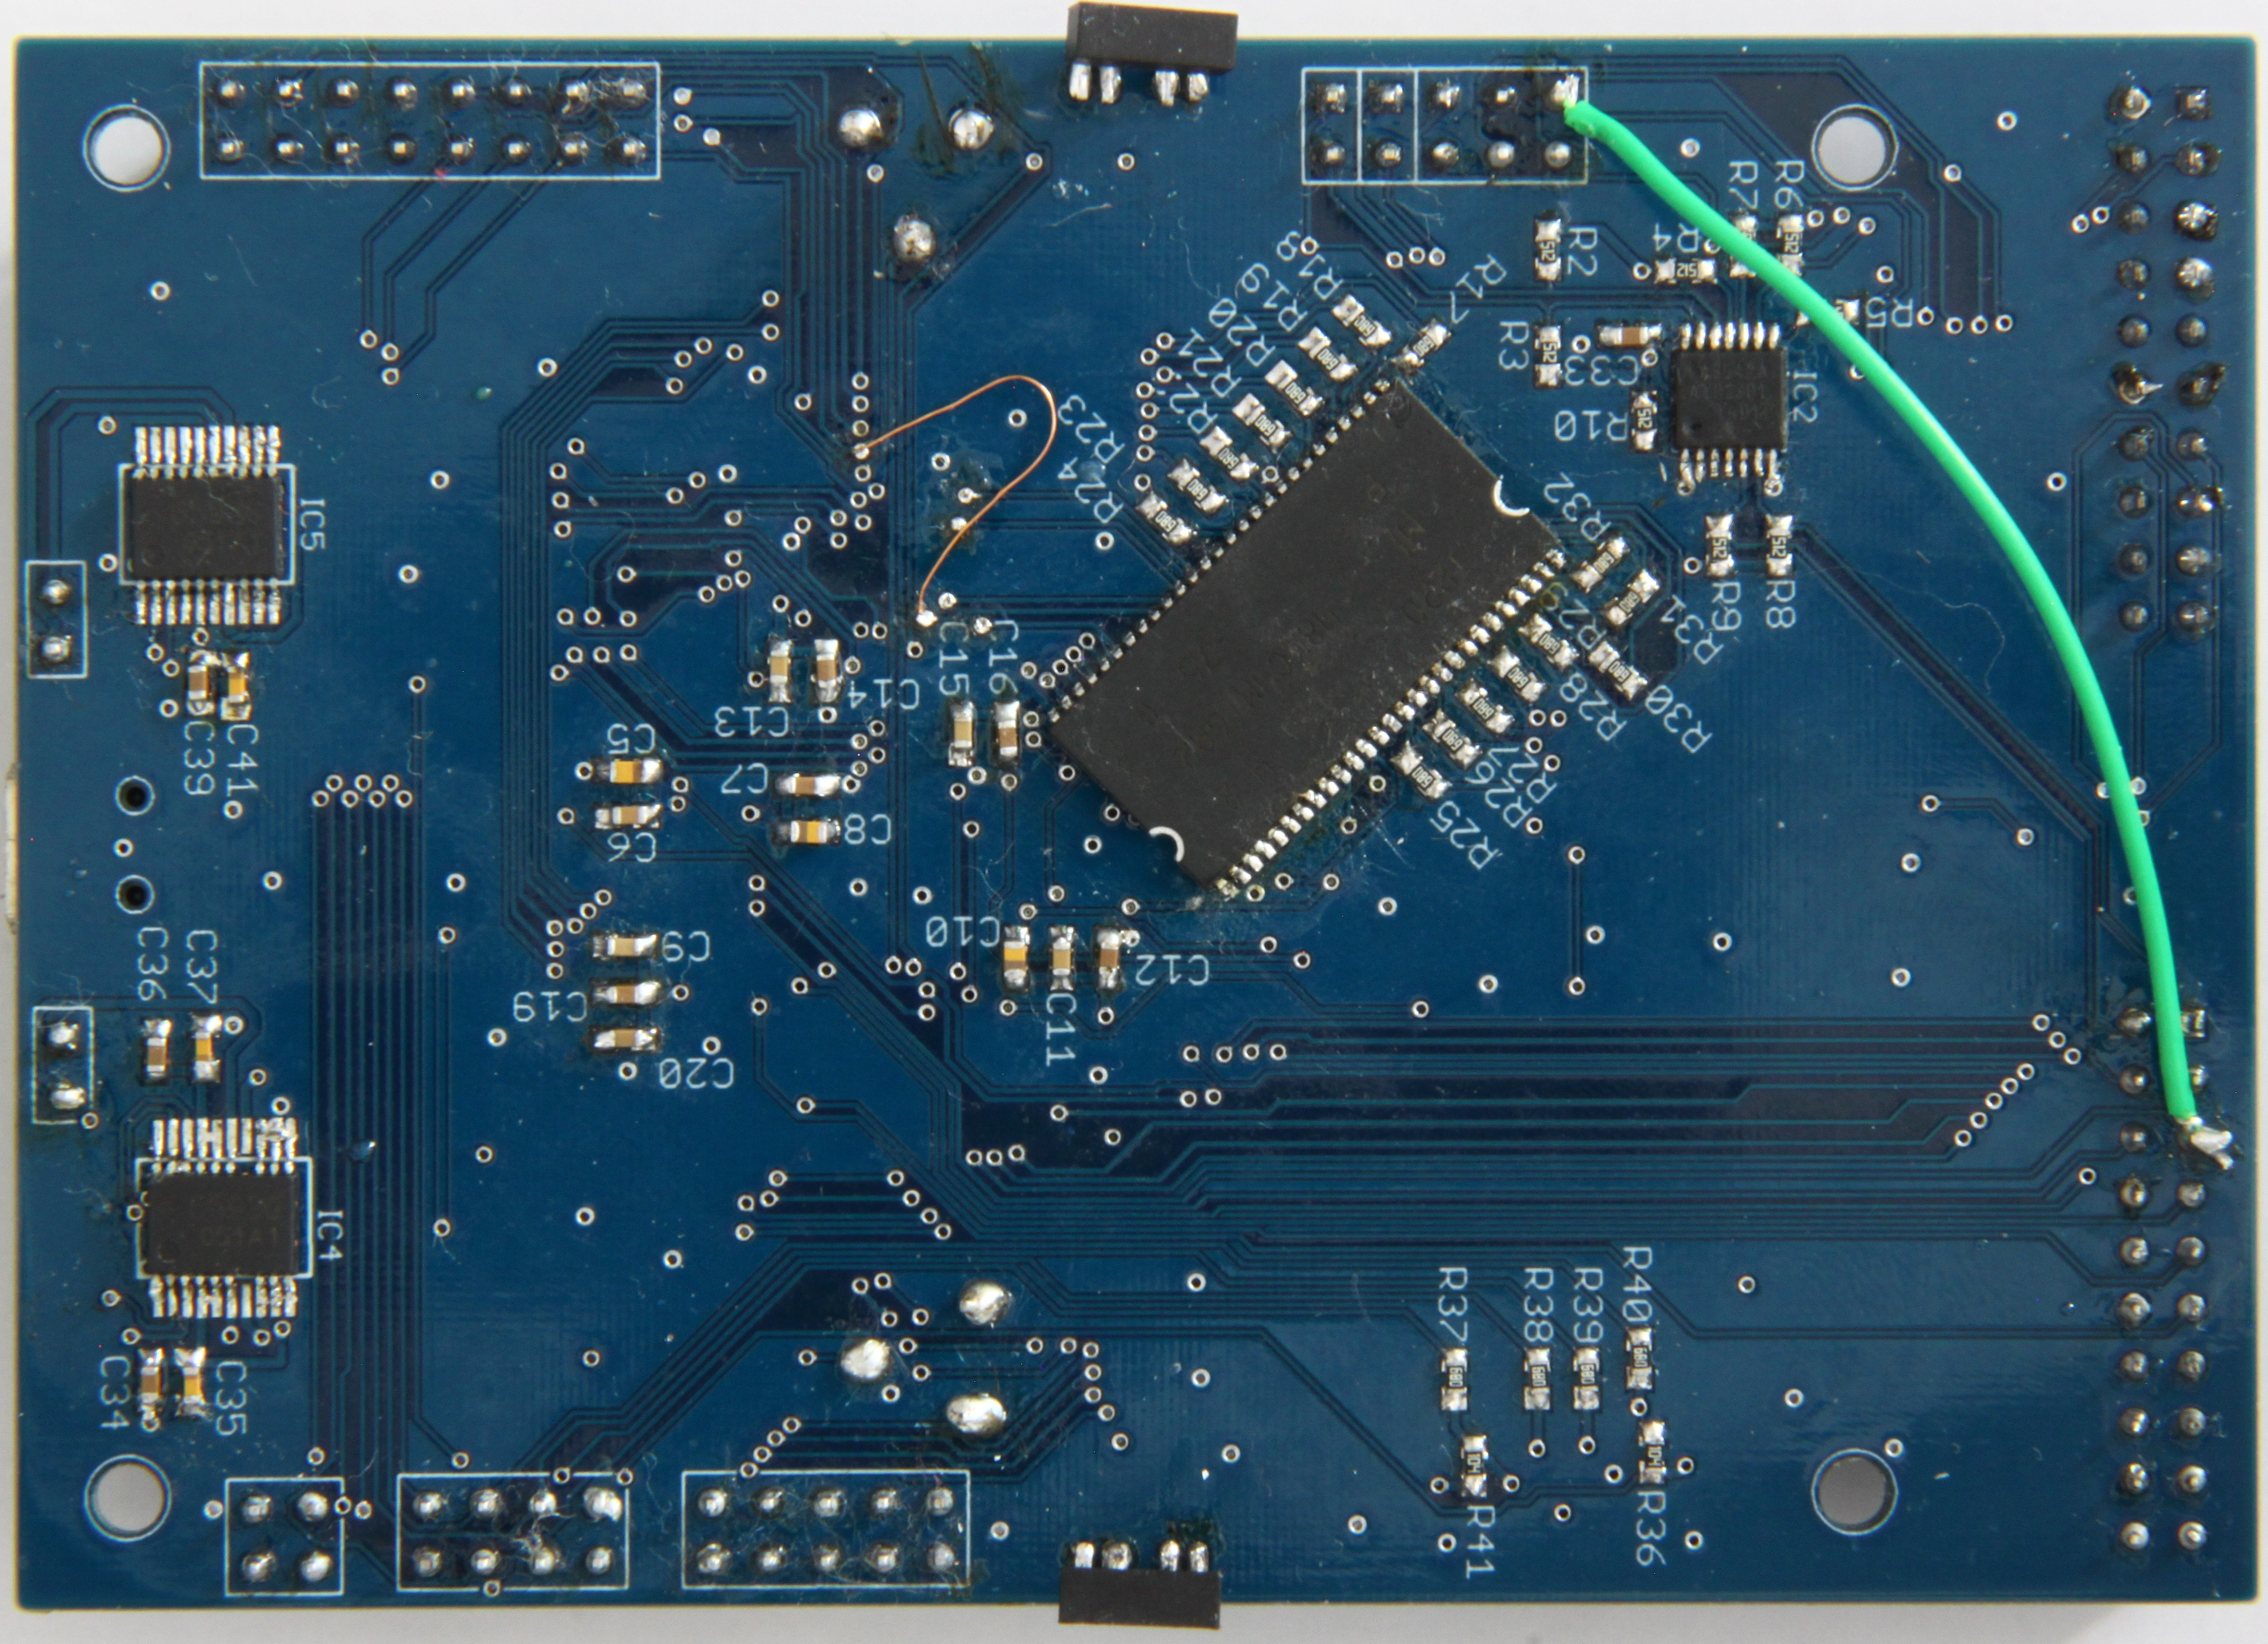
\includegraphics[width = \textwidth, keepaspectratio]{./Figures/PCB_Bottom.jpg} }
\caption{Pictures of the built PCB.}
\label{fig:PCB:Built}
\end{figure}
\section{Conclusions}

Overall, the hardware design and firmware is a success. A few minor faults were apparent on the PCB, but these were easily patched and caused no problem. Using a firmware test, the components are seen to be fully functional giving the UC3C full ability to control motors, cameras, \itc multiplexer, memory of both SD card (up to 2GB size) and external 4MB RAM. This provides a good platform for a manoeuvrable, stereoscopic image robot to be developed. 
%% ----------------------------------------------------------------
%% InvestigationVision.tex
%% ---------------------------------------------------------------- 
\chapter{Investigation into Vision Algorithms} \label{Chapter:InvestigationVision}
The Stereo vision algorithms sections to my Report \dots

Image registration classified into four 
reference BROWN but take from Registration of stereo and temporal images pdf in project/Documents
%%% ----------------------------------------------------------------
%% Results.tex
%% ---------------------------------------------------------------- 
\chapter{Results} \label{Chapter:Results}

\inote{A full test of the system I have got}
\inote{Summary of good and bad WITH EVIDENCE}
%% ----------------------------------------------------------------
%% Conclusions.tex
%% ---------------------------------------------------------------- 
\chapter{Conclusions and Further Work} \label{Chapter: Conclusions}
%\section{Conclusion}

%\inote{What I have accomplished}
This work has led to a tested device which is mobile and has the capability to perform stereoscopic image processing. The system has the following parts:

\begin{enumerate}
\item Motor driving
\item Stereoscopic Cameras
\item SD Card memory
\item SDRAM
\item Image Processing
\end{enumerate} 

The motor system is a simple, cheap method to move distances with reasonable accuracy. A better controller would allow variable speed and speed matching between motors. The system was shown to work to $4.5\%$ accuracy over a $300mm$ distance.

Stereo image pairs can be captured and stored on an SD card in a FAT32 file system. The SD card is also used for transferring images to and reading log files on a computer. Images are stored in QVGA format ($320px \times 240px$) as a Bitmap image. 

An additional 4MB of SDRAM memory is available to use on the robot allowing for large data arrays of the images to be kept in fast access RAM. The RAM is direct memory accessed (DMA) so operation is almost seamless from internal memory.

Multiple comparison algorithms have been investigated and compared using the same test images. It was clear that, although at a necessity of more computations, the normalised cross correlation is the best with regard to overall reliability. 

Range finding equations were then researched and derived, which use the characteristics of the camera and the separation distance between them to calculate distance to objects in view. The range finding capability was tested using MATLAB and it found that the system could not accurately calculate distances to objects. However, depth perception is possible even with low resolution cameras and small separation between them. A wide angle lens could be added to the system to more accurately measure distances but at the expense of reducing the maximum range.

The Fourier transform was also investigated and implemented. The system allows for a 2D array of a square image with dimensions of $2^{2n}\; $, where $n \in \mathbb{N}$, and is limited by RAM space and time. The transform is speed optimised and in tests proved to be fairly accurate. 

All aspects implemented on the robot have been shown to be functional. A faster processor would have been a good idea to use for image processing, but this could have developed other problems with the PCB. The Raspberry Pi or Steve Gunn's \textit{`L'Imperatrice'}, which both run a Linux operating system, would have been a good choice to remove the need for as much hardware design. Existing image processing libraries could then have been used to gain more functionality. 

Though some aspects of the specification were not fulfilled completely, the progress made during this project, and the challenges that have been overcome, provide a good platform for further development.
%Though the robots original application wasn't achieved, the end device is a base for a stereoscopic application. The system is a tested platform for future applications to be implemented on and additions can be made using the spare pins and bus connections on the PCB headers. 

The system could be used in future projects to develop more functionality. Wireless communications could be added to the system to allow a connection to the computer, and search algorithms can be implemented alongside distance calculations to make the robot aware of its surroundings. 
%\inote{What could be changed to make it better}
%\inote{Suggestions for further work}

\section{System Operation}

The system uses a debug USART available on J7 (57600bps, 8 data, 0 parity and 1 stop bit).

The system has two modes of operation, `Auto Run' and debug. By default, the Auto Run mode will run. Debug mode can be entered by the relevant command in the Auto Run procedure (see table \ref{table:AutoRun}) or by connecting Pin D23, available at Pin 1 of J9, to ground on system start. The state of the robot is shown by the LEDs. Table \ref{table:LEDs} shows the meaning of the LEDs.

Auto Run mode runs a set of commands located in \textit{``AutoRun.txt''} on the SD Card. If this file is not present, the system will run a default procedure defined in the code. A list of commands that can be run from this mode can be seen in table \ref{table:AutoRun}. The commands are specified by line. If an invalid command is found, the system will exit and run the \textit{System\_Error} loop. The  \textit{System\_Error} loop prints the status of all devices out once a second. By attaching a USART terminal, the error can be found.

Debug mode is a DOS-shell style terminal allowing the user to access methods and variables. This was used for development and debugging. A full list of commands can be seen in table \ref{table:Debug}. 

The final robot can be seen in figure \ref{fig:Robot:Complete}.

\begin{figure}
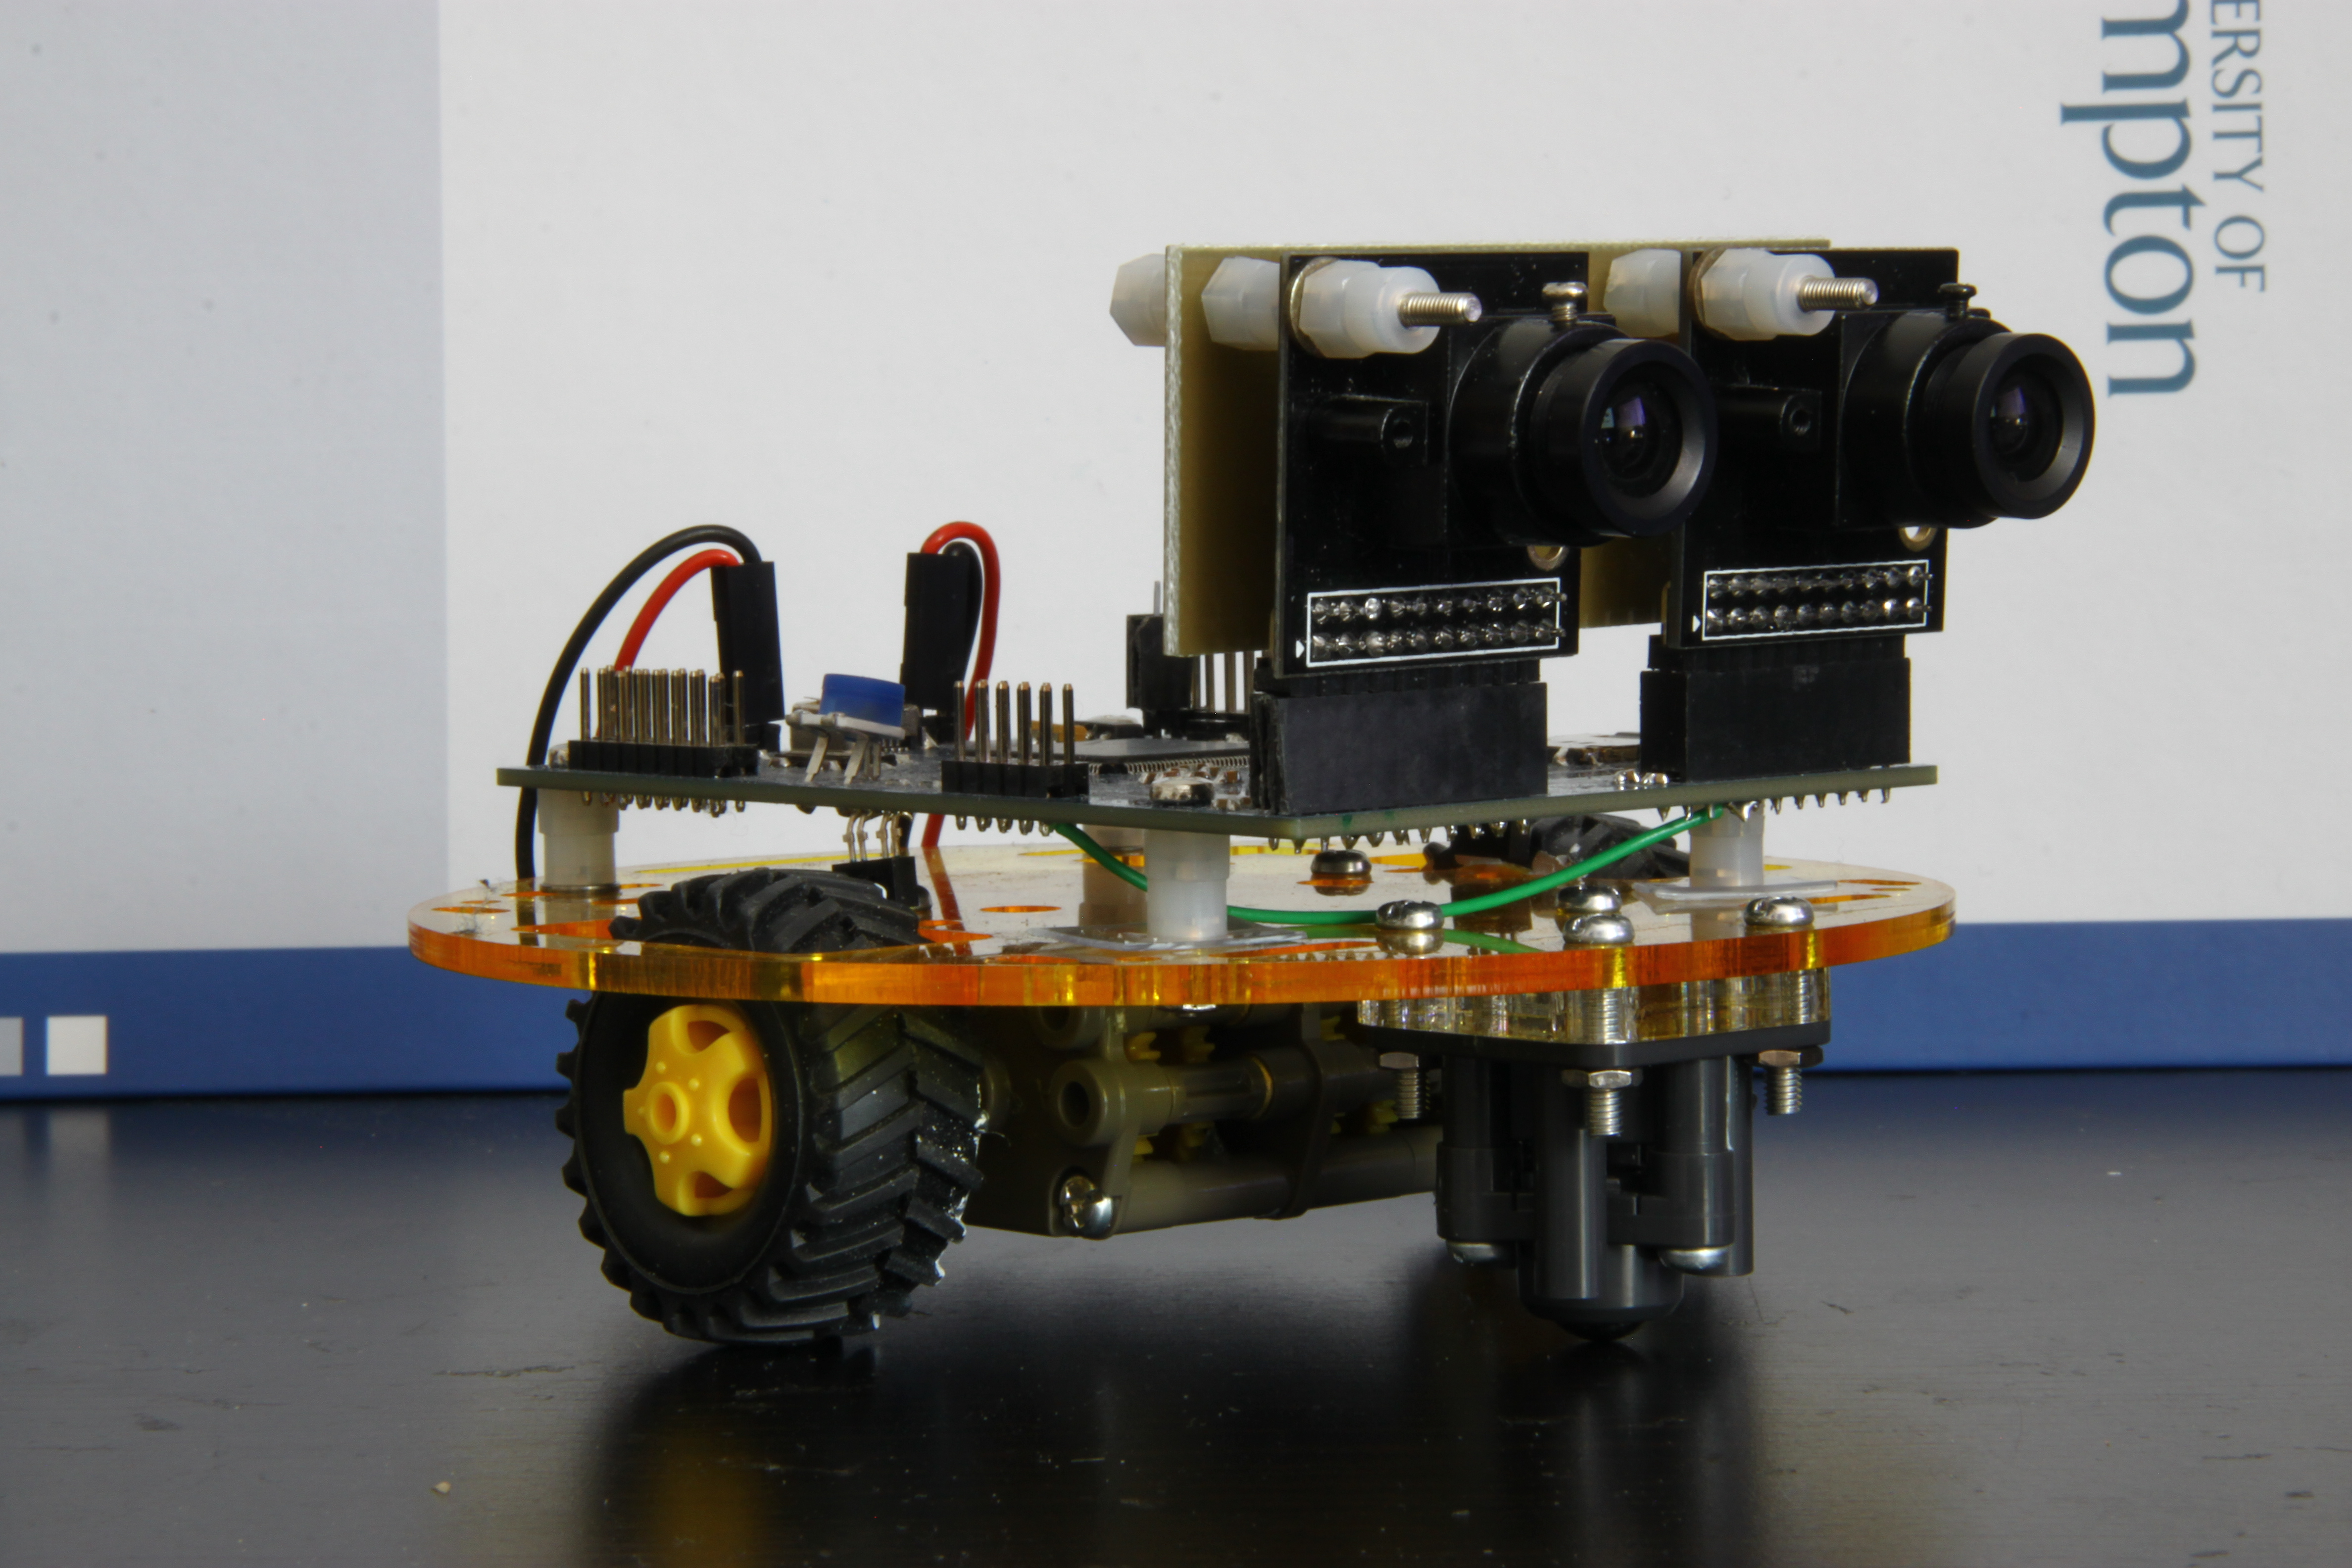
\includegraphics[width=\textwidth]{Figures/Robot.jpg}
\caption{The completed robot}
\label{fig:Robot:Complete}
\end{figure}

\begin{table}
\centering
\caption{Table showing the Auto Run commands implemented}
\label{table:AutoRun}
\begin{tabular}{ccc}\toprule
Command & 	Argument 			& 	Operation \\\toprule
B		&	int					&	Move backward by the argument value (millimetres) \\\midrule
F		&	int 				&	Move forward by the argument value (millimetres)\\\midrule
J		&	int					&	Jumps to the command specified (0 indexed)\\\midrule
P		&	N/A					&	Takes a stereo pair of photos\\\midrule
q		&	N/A					&	Quits Auto Run and enters debug mode\\\midrule
R		& 	int 			 	&	Rotates by argument (degrees)\\ \bottomrule
\end{tabular}
\end{table}

\begin{table}
\centering
\caption{Table showing the available debug commands}
\label{table:Debug}
\begin{tabular}{llp{10cm}}\toprule
Command & Argument & Operation \\\toprule
? && Shows the help prompt\\ \midrule
A && Runs the Auto Run procedure in debug mode\\ \midrule
B && Reads a Bitmap file and prints information \\ \midrule
c && converts the working buffer from integer to fixed point\\\midrule
C && Converts the working buffer from fixed point to integer\\\midrule
d && Saves the Working Buffer to ``Buffer\_results.csv'' \\ \midrule
D && Frees the Memory pointed to by the Working Buffer \\ \midrule
f && Reads ``Buffer.csv'' as a 2D Array of FFT\_SIZE by FFT\_SIZE\\ \midrule
g && Saves the Complex Buffer to ``Buffer\_Complex.csv'' \\\midrule
k && Prints the Complex Buffer \\ \midrule
m && Computes the Magnitude of the 1D FFT of the Working Buffer \\\midrule
M F &(int) & Drive Robot forward by (int) millimetres (negative number for reverse)\\\midrule
M L && Dive Left Wheel Forward a full rotation \\\midrule
M q && Resets Motors \\\midrule
M R && Drive Right Wheel Forward a full rotation \\\midrule
M T &(int) & Rotate Robot by (int) degrees (positive turns Clockwise)\\\midrule
o && Displays the fixed point value for (int)1 \\\midrule
P && Takes and stores Stereo Photos \\ \midrule
r && displays the contents of the working buffer\\\midrule
R && Reads contents of ``signal.bin'', representing 1D Signal. Integers, Big Endian\\\midrule
T && Reads contents of ``signal2d.bin'', representing 2D Signal. \\ \midrule
s && saves the working buffer\\\midrule
S && Saves the image in memory to a Bitmaps \\\midrule
v && Prints the status variables \\ \midrule
1 && computes the One Dimensional FFT of the working buffer. Returns magnitude.\\\midrule
2 && Computes the Magnitude of the Two Dimensional FFT of the Working Buffer. \\ \midrule
3 && Computes the Complex 2D FFT of the working buffer and stores it in the Complex Buffer \\ \bottomrule
\end{tabular}
\end{table}

\begin{table}
\centering
\caption{Table show the meaning of the LED lights. F - Flashing, X - Don't Care}
\label{table:LEDs}
\begin{tabular}{ccccccc}\toprule
\multicolumn{6}{c}{LED} 						& Meaning\\ \cmidrule{1-6}
MOTOR 	& 2		& 3 	& 4 	& 5 	& 6 	& \\ \toprule
Off		& Off	& Off	& Off	& Off	& Off	& System Initialising \\ \midrule
On		& X		& X		& X		& X		& X		& Robot moving\\\midrule
Off		& X		& X		& X		& X		& X		& Robot not moving\\\midrule
X		& On	& On	& On	& X		& X 	& System in Debug Mode \\\midrule
X		& X		& X		& X		& On	& X		& Left Wheel on a `Tab'	\\\midrule
X		& X		& X		& X		& Off	& X		& Left Wheel not on a `Tab'	\\\midrule
X		& X		& X		& X		& X 	& On	& Right Wheel on a `Tab'	\\\midrule
X		& X		& X		& X		& X		& Off	& Right Wheel not on a `Tab'	\\\midrule
Off		& On	& Off	& Off	& X		& X		& Auto Run Mode - Robot taking photos	\\\midrule
On		& Off	& On	& Off	& X		& X		& Auto Run Mode - Robot rotating	\\\midrule
On		& Off	& Off	& On	& X		& X		& Auto Run Mode - Robot moving\\\midrule
Off		& F		& Off	& Off	& X		& X		& System Error - Generic\\\midrule
Off		& F		& F		& X		& X		& X		& System Error - SD Card Error\\\midrule
Off		& F		& X		& F		& X		& X		& System Error - Camera Error\\ \bottomrule
\end{tabular}
\end{table}


\bibliographystyle{ecs}
\addtotoc{References}
\bibliography{ECS}
%TC:ignore
\appendix
%% ----------------------------------------------------------------
%% AppendixA.tex Circuit Diagrams
%% ---------------------------------------------------------------- 
\chapter{Project Brief} \label{Chapter:Appendix:Brief}
\includepdf[frame = true, pagecommand=\section{Project Brief}\label{pdf:ProjectBrief}, offset = -1in -1.5in, scale = 0.8]{Figures/ProjectBrief_hl13g10.pdf}
%% ----------------------------------------------------------------
%% AppendixD.tex
%% ---------------------------------------------------------------- 
\chapter{Gantt Charts} \label{Chapter:AppendixD:Gannt}

\begin{figure}
\centering
\includegraphics[angle = 90,height=\textheight]{Figures/Gantt.pdf} 
\caption{Gantt Chart of how time was decided to be spent at the beginning of the project}
\label{fig:Gantt:1}
\end{figure}
\clearpage
\begin{figure}
\centering
\includegraphics[angle = 90, height=\textheight]{Figures/Gantt2.pdf} 
\caption{Gantt Chart of how time during term two was decided to be spent after interim report hand-in}
\label{fig:Gantt:2}
\end{figure}

\begin{figure}
\centering
\includegraphics[angle = 90, height=\textheight]{Figures/Gantt3.pdf} 
\caption{Gantt Chart of how time was actually spent throughout the project}
\label{fig:Gantt:3}
\end{figure}
%% ----------------------------------------------------------------
%% AppendixA.tex Circuit Diagrams
%% ---------------------------------------------------------------- 
\chapter{Circuit Diagrams} \label{Chapter:AppendixA:CircuitDiagrams}
\section{OV7670 Breakout Board Schematic}\label{sch:OV7670}
\begin{figure}[ht!]
\centering
\includegraphics[angle=90,width=\textwidth,height=\textheight-10cm,keepaspectratio]{Figures/OV7670_Schematic.jpg} 
\caption{The circuit diagram for the OV7670 breakout board}
\label{OV7670_Schematic}

\end{figure}
\clearpage
\section{Il Matto and Dual Camera Schematic}\label{sch:IlMatto:Cameras}
\begin{figure}[ht!]
\centering
\includegraphics[angle = 90, width=\textwidth,height=\textheight,keepaspectratio]{Figures/IlMattoCamera_CircuitDiagram.png} 
\caption{The circuit diagram for Dual Cameras using the Il Matto Board}
\label{sch:DualCam_Schematic}
\end{figure}
\clearpage

\section{The Columbus Circuit Diagram} \label{sch:Columbus:CircuitDiagram}
\begin{figure}[ht!]
\centering
\includegraphics[angle = 90, width=\textwidth,height=\textheight,keepaspectratio]{./Figures/ColumbusCircuitPage1.png}
\caption{The Columbus Circuit Diagram Page 1}
\label{sch:Columbus_Schematic:1}
\end{figure}

\begin{figure}[ht!]
\centering
\includegraphics[angle = 90, width=\textwidth,height=\textheight,keepaspectratio]{./Figures/ColumbusCircuitPage2.png}
\caption{The Columbus Circuit Diagram Page 2}
\label{sch:Columbus_Schematic:2}
\end{figure}

\begin{figure}[ht!]
\centering
\includegraphics[angle = 90, width=\textwidth,height=\textheight,keepaspectratio]{./Figures/ColumbusCircuitPage3.png}
\caption{The Columbus Circuit Diagram Page 3}
\label{sch:Columbus_Schematic:3}
\end{figure}

\begin{figure}[ht!]
\centering
\includegraphics[angle = 90, width=\textwidth,height=\textheight,keepaspectratio]{./Figures/ColumbusCircuitPage4.png}
\caption{The Columbus Circuit Diagram Page 4}
\label{sch:Columbus_Schematic:4}
\end{figure}

\begin{figure}[ht!]
\centering
\includegraphics[angle = 90, width=\textwidth,height=\textheight,keepaspectratio]{./Figures/ColumbusCircuitPage5.png}
\caption{The Columbus Circuit Diagram Page 5}
\label{sch:Columbus_Schematic:5}
\end{figure}

\begin{figure}[ht!]
\centering
\includegraphics[angle = 90, width=\textwidth,height=\textheight,keepaspectratio]{./Figures/ColumbusCircuitPage6.png}
\caption{The Columbus Circuit Diagram Page 6}
\label{sch:Columbus_Schematic:6}
\end{figure}


%% ----------------------------------------------------------------
%% AppendixA.tex Circuit Diagrams
%% ---------------------------------------------------------------- 
\chapter{PCB Design} \label{Appendix:PCB}
\section{PCB Top Side}
\begin{figure}[ht!]
\centering
\includegraphics[angle=90,width=\textwidth,height=\textheight-5cm,keepaspectratio]{Figures/ColumbusPCBTop_GP.png} 
\caption{The top side of the CAD design of the PCB}
\label{fig:PCB:Eagle:Top}
\end{figure}
\clearpage
\section{PCB Layer 2}
\begin{figure}[ht!]
\centering
\includegraphics[angle=90,width=\textwidth,height=\textheight-5cm,keepaspectratio]{Figures/layer2.png} 
\caption{Layer 2 of the CAD design of the PCB}
\label{fig:PCB:Eagle:Bottom}
\end{figure}
\clearpage
\section{PCB Layer 3}
\begin{figure}[ht!]
\centering
\includegraphics[angle=90,width=\textwidth,height=\textheight-5cm,keepaspectratio]{Figures/layer3.png} 
\caption{Layer 3 of the CAD design of the PCB}
\label{fig:PCB:Eagle:Bottom}
\end{figure}
\clearpage
\section{PCB Bottom Side}
\begin{figure}[ht!]
\centering
\includegraphics[angle=90,width=\textwidth,height=\textheight-5cm,keepaspectratio]{Figures/ColumbusPCBBottom_GP.png} 
\caption{The bottom side of the CAD design of the PCB}
\label{fig:PCB:Eagle:Bottom}
\end{figure}
\clearpage
%% ----------------------------------------------------------------
%% AppendixA.tex Circuit Diagrams
%% ---------------------------------------------------------------- 
\chapter{Costings} \label{Appendix:Costings}

\begin{table}
\centering
\begin{tabular}{|c|p{2cm}|c|c|c|} \hline
Component	&	Cost per unit (\pounds)	& Quantity 	&	Cost (\pounds)		&	Source		\\ \hline
PCB			&	205						&	1		&	205					&	PCBCart		\\
Capactiors	&	0.155 					& 	43		& 	6.67 				& 	Farnell 	\\
Clock 		& 	1.48					& 	1		&	1.48 				& 	Farnell		\\
Diode		&	0.48					&	1		&	0.48				&	Farnell 	\\
Headers		&	0.51 					&	5		&	2.55				&	Farnell 	\\
I2C Mux PCA9542A &	0.81				&	1		&	0.81				&	Farnell		\\
LEDs 		&	0.158					&	7		& 	1.11 				&	Farnell		\\
Micro SD Card &	4						&	1		&	4.00 				&	Amazon 		\\
Micro SD Card Connector & 2.04			&	1		&	2.04				&	Farnell		\\
AT32UC3C0512C	&15.39					&	1		&	15.39				&	Farnell		\\
TB6593FNG 	&	1.07 					&	2 		&	2.14 				&	Farnell 	\\
Motors  	&	0.42					&	2		&	0.84				&	Rapid 		\\
TCRT1010	& 	0.94 					&	2		&	1.88 				&	Farnell 	\\
OV7670		&	17						&	2		&	34.00				& 				\\
Potentiometer	&	0.43				&	2		&	0.86				&	Farnell 	\\
Resistors	&	0.066 					& 	46		&	3.04 				&	Farnell 	\\
MT48LC4M16A2P	& 3.24  				& 	1		&	3.24 				&	Farnell		\\
Switch		&	0.45					&	1		&	0.45				&	Farnell 	\\
USB Socket	&	0.84 					&	1		& 	0.84 				&	Farnell 	\\
LM1117MP	&	1.03					&	1		&	1.03	 			&	Farnell		\\ \hline \cline{3-4}
\multicolumn{2}{c|}{ }					& Total Cost  & \pounds 287.84		&	\multicolumn{1}{|c}{ }			\\ \cline{3-4}
\end{tabular}
\caption{A table of all components used and their costs.}
\label{table:Costings}
\end{table}
%% ----------------------------------------------------------------
%% Appendix_TestCode.tex Test Code
%% ---------------------------------------------------------------- 
\chapter{PCB Test Code} \label{Appendix:TestCode}

\section{USART Test Code}
\lstinputlisting[style=C,caption=USART Test Code,label={lst:USARTTestCode},frame=single,numbers=left,tabsize=2,breaklines=true, firstline=110,lastline=121]{../Code/ColumbusTest/ColumbusTest/src/main.c}
\section{SD Card Test Code}
\lstinputlisting[style=C,caption=SD Test Code,label={lst:SDTestCode},frame=single,numbers=left,tabsize=2,breaklines=true, firstline=124,lastline=196]{../Code/ColumbusTest/ColumbusTest/src/main.c}
\section{LED Test Code}
\lstinputlisting[style=C,caption=SDRAM Test Code,label={lst:LEDTestCode},frame=single,numbers=left,tabsize=2,breaklines=true, firstline=197,lastline=215]{../Code/ColumbusTest/ColumbusTest/src/main.c}
\section{SDRAM Test Code}
\lstinputlisting[style=C,caption=SDRAM Test Code,label={lst:SDRAMTestCode},frame=single,numbers=left,tabsize=2,breaklines=true, firstline=217,lastline=258]{../Code/ColumbusTest/ColumbusTest/src/main.c}
\section{\itc Test Code}
\lstinputlisting[style=C,caption=\itc Test Code,label={lst:TWITestCode},frame=single,numbers=left,tabsize=2,breaklines=true, firstline=268,lastline=315]{../Code/ColumbusTest/ColumbusTest/src/main.c}
\section{Camera Test Code}
\lstinputlisting[style=C,caption=Camera Test Code,label={lst:CameraTestCode},frame=single,numbers=left,tabsize=2,breaklines=true, firstline=316,lastline=338]{../Code/ColumbusTest/ColumbusTest/src/main.c}
\section{Motor Test Code}
\lstinputlisting[style=C,caption=Motor Test Code,label={lst:MotorTestCode},frame=single,numbers=left,tabsize=2,breaklines=true, firstline=339,lastline=346]{../Code/ColumbusTest/ColumbusTest/src/main.c}
%% ----------------------------------------------------------------
%% AppendixC.tex
%% ---------------------------------------------------------------- 
\chapter{Contents of Files} \label{Appendix:Contents}
\begin{itemize}
\item Contents.txt
\item encc\_matlab.zip
\item Harris.zip
\item README
\item stereo\_example.zip
\item TcfTransactionLog.csv
\item texput.log
\item CircuitDiagrams
\begin{itemize}
\item Project
\begin{itemize}
\item eagle.epf
\item project.bcl.pdf
\item project.brd
\item project.pdf
\item project.pro
\item project.sch
\item project.tcl.pdf
\end{itemize}
\end{itemize}
\item Code
\begin{itemize}
\item AnalogueComparator
\item ColumbusTest
\item DualCamera\_UI
\item DualOV7670
\item FatFS
\item MotorDriver
\item OV7670+AVR+TFT-Jian
\item OV7670seblov
\item OV7670\_FATFS
\item PhotoViewer
\item PORTAtoSPI
\item SDCard
\item SDTest
\item SerialToI2C
\item The\_Columbus
\end{itemize}
\item Documents
\begin{itemize}
\item 0.3M Sensor OV7670.pdf
\item AT32UC3.pdf
\item ATmega644P.pdf
\item Costings.xlsx
\item EffectiveCornerMatching.pdf
\item ExampleProjectWriteUp.pdf
\item Iterative\_Image\_Registration.pdf
\item lm1117.pdf
\item MT48LC16M4A2.pdf
\item PCA9542A.pdf
\item PCBChanges.txt
\item RegistationofStereoandTemporalImages.pdf
\item research.txt
\item SDRAM.pdf
\item Stereoscopy\_(Mrovlje).pdf
\item SzeliskiBook.pdf
\item TB6593FNG.pdf
\item tcrt1000.pdf
\end{itemize}
\item Matlab
\begin{itemize}
\item archive
\item Range\_Test\_Images
\end{itemize}
\item ProjectBrief

\item Report
\begin{itemize}
\item Figures
\end{itemize}
\item SDCard
\end{itemize} 
        

\include{Appendix_Bitmap}
%% ----------------------------------------------------------------
%% AppendixA.tex Circuit Diagrams
%% ---------------------------------------------------------------- 
\chapter{Range Finding Derivations} \label{Appendix:Range}
\begin{figure}
\includegraphics[width=\textwidth,height=\textheight,keepaspectratio]{Figures/problem1.pdf}
\caption{Problem 1 - Object is between the cameras}
\label{problem_between}
\end{figure}

\section{Object is between the Cameras}
Derivation from \cite{Mrovlje:Distance_Stereoscopic}.
\begin{equation} \label{eq:B}
B = B_{1} + B_{2} = D\tan(\varphi_{1}) + D\tan(\varphi_{2})
\end{equation}

\begin{equation} \label{eq:D}
D = \frac{B}{\tan(\varphi_{1}) + \tan(\varphi_{2})}
\end{equation}


%\begin{figure}
%\includegraphics[width=\textwidth,height=\textheight,keepaspectratio]{Figures/left_simplified.png}
%\caption{Problem 1 : Left Camera Simplified}
%\label{Left_Simplified}
%\end{figure}

\begin{equation} \label{eq:phi}
D\tan\left(\frac{\varphi_{0}}{2}\right) = \frac{x_{0}}{2}
\end{equation}

\begin{equation} \label{eq:phi1}
D\tan(\varphi_1) = x_1
\end{equation}

Dividing \eqref{eq:phi1} by \eqref{eq:phi}

\begin{equation} \label{eq:tanovertan}
\frac{\tan(\varphi_1)}{\tan(\frac{\varphi_0}{2})} = \frac{2x_1}{x_0}
\end{equation}

\begin{equation} \label{eq:phionesolved}
\tan(\varphi_1) = \frac{2x_1\tan(\frac{\varphi_0}{2})}{x_0}
\end{equation}

This can also be shown for the right camera:

\begin{equation} \label{eq:phitwosolved}
\tan(\varphi_2) = \frac{-2x_2\tan(\frac{\varphi_0}{2})}{x_0}
\end{equation}

Substituting Equations \eqref{eq:phionesolved} and \eqref{eq:phitwosolved} into \eqref{eq:D} gives

\begin{equation} \label{eq:Distance1}
D = \frac{Bx_0}{2\tan(\frac{\varphi_0}{2})(x_1 - x_2)}
\end{equation}


\section{Object is to the same side in each Camera}
Derivation is based on the derivation from \cite{DistanceEstimation}. Using Figure \ref{problem_toleft}:

\begin{equation} \label{eq:p2:tanphi1}
D.\tan(\varphi_{1}) = x_{1}
\end{equation}

\begin{equation} \label{eq:p2:tanphi0}
D.\tan\left(\frac{\varphi_{0}}{2}\right) = \frac{x_{0}}{2}
\end{equation}

\begin{equation} \label{eq:p2:tanphi0and1}
\frac{\tan(\varphi_{1})}{\tan(\frac{\varphi_0}{2})} = \frac{2x_1}{x_0}
\end{equation}

\begin{equation} \label{eq:p2:phi1:ap}
\varphi_1 = \arctan\left(\frac{2x_1}{x_0}\tan\left(\frac{\varphi_0}{2}\right)\right)
\end{equation}

and similarly
\begin{equation} \label{eq:p2:phi2:ap}
\varphi_2 = \arctan\left(\frac{2x_2}{x_0}\tan\left(\frac{\varphi_0}{2}\right)\right)
\end{equation}
\begin{equation} \label{eq:p2:theta}
\theta = \varphi_2 - \varphi_1
\end{equation}

Using the sine equality rule:

\begin{equation} \label{eq:p2:sineeq}
\frac{R}{\sin(\frac{\pi}{2} - \varphi_2)} = \frac{B}{\sin(\theta)}
\end{equation}

\begin{equation} \label{eq:p2:R}
R = B.\frac{\sin(\frac{\pi}{2} - \varphi_2)}{\sin(\theta)} = B \frac{\cos(\varphi_2)}{\sin(\theta)}
\end{equation}

\begin{equation} \label{eq:p2:DeqR}
D = \cos(\varphi_1).R
\end{equation}
Substituting \eqref{eq:p2:theta} into \eqref{eq:p2:R}, and then into \eqref{eq:p2:DeqR}:

\begin{equation} \label{eq:p2:DeqB}
D = B.\frac{\cos(\varphi_2).\cos(\varphi_1)}{sin(\varphi_2 - \varphi_1)}
\end{equation}

Where $\varphi_1$ is defined in Equation \eqref{eq:p2:phi1:ap} and $\varphi_2$ is defined in Equation \eqref{eq:p2:phi2:ap}. 

\begin{figure}
\includegraphics[width=\textwidth,height=\textheight,keepaspectratio]{Figures/problem2.pdf}
\caption{Problem 2 - Object is to the same side in both cameras}
\label{problem_toleft}
\end{figure}

\section{Object is in front of a Camera}
The distance, $D$, in this problem is given by:

\begin{equation} \label{eq:p3:D}
D = B \tan\left(\frac{\pi}{2} - \varphi_{2}\right)
\end{equation}
Where $\varphi_2$ can be found from Equation \ref{eq:p2:phi2}. 
\begin{figure}
\includegraphics[width=\textwidth,height=\textheight,keepaspectratio]{Figures/problem3.pdf}
\caption{Problem 3 - Object is directly in front of a camera}
\label{fig:problem_infront}
\end{figure}
%\include{Appendix_Code}
%TC:endignore
\backmatter

\end{document}
%% ----------------------------------------------------------------
